\documentclass[../../main/main.tex]{subfiles}
\graphicspath{{./figures/}}

\dominitoc
\faketableofcontents

\makeatletter
\renewcommand{\@chapapp}{M\'ecanique -- chapitre}
\makeatother

\toggletrue{student}
% \HideSolutionstrue
% \toggletrue{corrige}
% \renewcommand{\mycol}{black}
\renewcommand{\mycol}{gray}

\begin{document}
\setcounter{chapter}{4}

\chapter{Mouvement de particules charg\'ees}

\vspace*{\fill}

\begin{prgm}
	\small
	\begin{tcb}*(ror)"know"{Savoirs}
		\begin{itemize}
			\item Force de Lorentz exercée sur une charge
			      ponctuelle ; champs électrique et magnétique~; puissance de la force
			      de Lorentz.
		\end{itemize}
	\end{tcb}
	\begin{tcb}*(ror)"how"{Savoir-faire}
		\begin{itemize}
			\item Évaluer les ordres de grandeur des forces électrique
			      ou magnétique et les comparer à ceux des forces gravitationnelles.
			\item Justifier qu'un champ électrique peut modifier l'énergie cinétique
			      d'une particule alors qu'un champ magnétique peut courber la
			      trajectoire sans fournir d'énergie à la particule.
			\item Mouvement d'une particule chargée dans un champ $\Ef$
			      uniforme~:
			      \begin{itemize}
				      \item Mettre en équation le mouvement et le caractériser comme un
				            mouvement à vecteur $\af$ constant~;
				      \item Effectuer un bilan énergétique pour déterminer la valeur de
				            la vitesse d'une particule chargée accélérée par une
				            différence de potentiel.
			      \end{itemize}
			\item Mouvement d'une particule chargée dans un champ $\Bf$
			      uniforme pour $\vfo \perp \Bf$~: déterminer le rayon de la
			      trajectoire et le sens de parcours.
		\end{itemize}
	\end{tcb}
\end{prgm}

% \vspace*{\fill}

% \newpage

\vspace*{\fill}
\minitoc
\vspace*{\fill}

\newpage

\vspace*{\fill}
\begin{boxes}
	\begin{tcb}(defi)<lftt>{Liste des définitions}
		\tcblistof[\paragraph*]{defi}{\hspace*{6pt}}
	\end{tcb}
	\begin{tcb}(rapp)<lftt>{Liste des rappels}
		\tcblistof[\paragraph*]{rapp}{\hspace*{6pt}}
	\end{tcb}
	\begin{tcb}(prop)<lftt>{Liste des propriétés}
		\tcblistof[\paragraph*]{prop}{\hspace*{6pt}}
	\end{tcb}
	% \begin{tcb}(coro)<lftt>{Liste des corollaires}
	% 	\tcblistof[\paragraph*]{coro}{\hspace*{6pt}}
	% \end{tcb}
	\begin{tcb}(demo)<lftt>{Liste des démonstrations}
		\tcblistof[\paragraph*]{demo}{\hspace*{6pt}}
	\end{tcb}
	% \begin{tcb}(inte)<lftt>{Liste des interprétations}
	% 	\tcblistof[\paragraph*]{inte}{\hspace*{6pt}}
	% \end{tcb}
	% \begin{tcb}(tool)<lftt>{Liste des outils}
	% 	\tcblistof[\paragraph*]{tool}{\hspace*{6pt}}
	% \end{tcb}
	% \begin{tcb}(nota)<lftt>{Liste des notations}
	% 	\tcblistof[\paragraph*]{nota}{\hspace*{6pt}}
	% \end{tcb}
	% \begin{tcb}(appl)<lftt>{Liste des applications}
	% 	\tcblistof[\paragraph*]{appl}{\hspace*{6pt}}
	% \end{tcb}
	\begin{tcb}(rema)<lftt>{Liste des remarques}
		\tcblistof[\paragraph*]{rema}{\hspace*{6pt}}
	\end{tcb}
	% \begin{tcb}(exem)<lftt>{Liste des exemples}
	% 	\tcblistof[\paragraph*]{exem}{\hspace*{6pt}}
	% \end{tcb}
	\begin{tcb}(ror)<lftt>{Liste des points importants}
		\tcblistof[\paragraph*]{ror}{\hspace*{6pt}}
	\end{tcb}
	% \begin{tcb}(impo)<lftt>{Liste des erreurs communes}
	% 	\tcblistof[\paragraph*]{impo}{\hspace*{6pt}}
	% \end{tcb}
\end{boxes}
\vspace*{\fill}
\newpage

\section{Champs électrique et magnétique}
\subsection{Champ électrique}
\begin{tcb*}[sidebyside, righthand ratio=.3](defi){Champ électrique}
	Un champ électrique $\Ef(\Mr,t)$ est un champ de vecteurs créé par des
	charges électriques et par des variations temporelles du champ magnétique.
	\bigbreak
	\tcblower
	\tcbsubtitle{\fatbox{Unités}}
	\psw{
		\[
			\norm{\Ef(\Mr,t)} \qMath{en} \si{V.m^{-1}}
		\]
	}
	\vspace{-15pt}
\end{tcb*}

\noindent
\begin{minipage}{0.65\linewidth}
	La manière la plus simple pour créer un champ électrique est de constituer un
	condensateur avec deux armatures métalliques de surface $S$. On a alors
	\[\Ef = \frac{1}{\epo} \frac{q}{S}\uz\]
	avec la $\epo$ permittivité diélectrique du vide.
	\bigbreak
	$\Ef$ va des \textbf{charges positives aux négatives}. On le verra, il indique
	le \textbf{sens de la force subie par une charge positive}.
\end{minipage}
\hfill
\begin{minipage}{0.33\linewidth}
	\begin{center}
		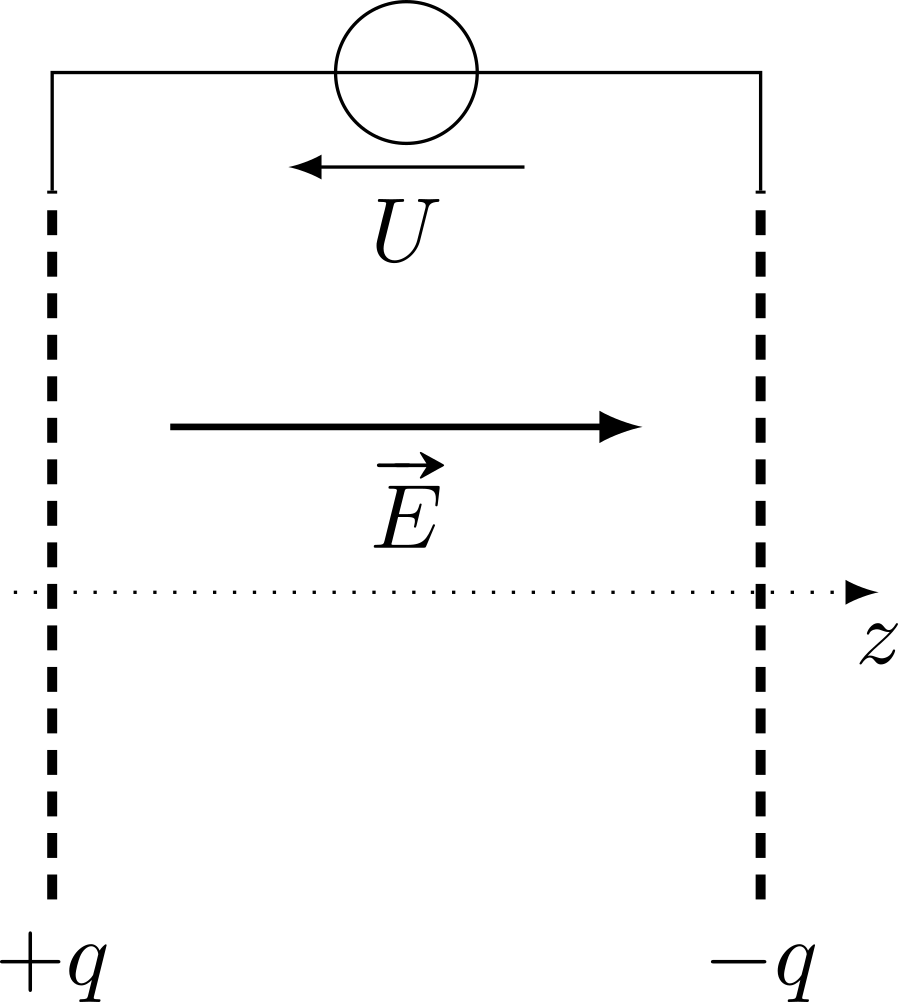
\includegraphics[width=.7\linewidth]{condo_base}
		\captionsetup{justification=centering}
		\captionof{figure}{Condensateur et champ électrique}
		\label{fig:condo}
	\end{center}
\end{minipage}

\begin{tcb*}(odgr)<lftt>'l'{Champs électriques}
	\begin{itemize}[label=$\diamond$]
		\item À l'intérieur d'un condensateur en TP, on a environ
		      \SI{10}{V.mm^{-1}}, soit \SI{10}{kV.m^{-1}}
		\item À la surface de la Terre, le champ électrique est d'environ
		      \SI{e2}{V.m^{-1}}
		\item Le champ électrique créé lors d'un orage est d'environ
		      \SI{e4}{V.m^{-1}}
		\item Le champ électrique pour la téléphonie mobile est d'environ
		      \SI{50}{V.m^{-1}}
	\end{itemize}
\end{tcb*}

\subsection{Champ magnétique}
\begin{tcb*}[sidebyside, righthand ratio=.3](defi){Champ magnétique}
	Un champ magnétique $\Bf(\Mr,t)$ est un champ de vecteurs créé par des
	courants électriques et par des variations temporelles du champ électrique.
	\tcblower
	\tcbsubtitle{\fatbox{Unités}}
	\psw{
		\[\norm{\Bf(\Mr,t)} \qMath{en} \mathrm{Tesla} \,(\si{T})\]
	}
	\vspace{-15pt}
\end{tcb*}

\noindent
\begin{minipage}{0.65\linewidth}
	La manière la plus simple pour créer un champ magnétique est de constituer
	une bobine, par enroulement de $N$ spires d'un fil métallique sur une
	longueur $L$. On a alors
	\[\Bf = \muo i\frac{N}{L}\,\uz\]
	avec la $\muo$ perméabilité magnétique du vide.
\end{minipage}
\hfill
\begin{minipage}{0.33\linewidth}
	\begin{center}
		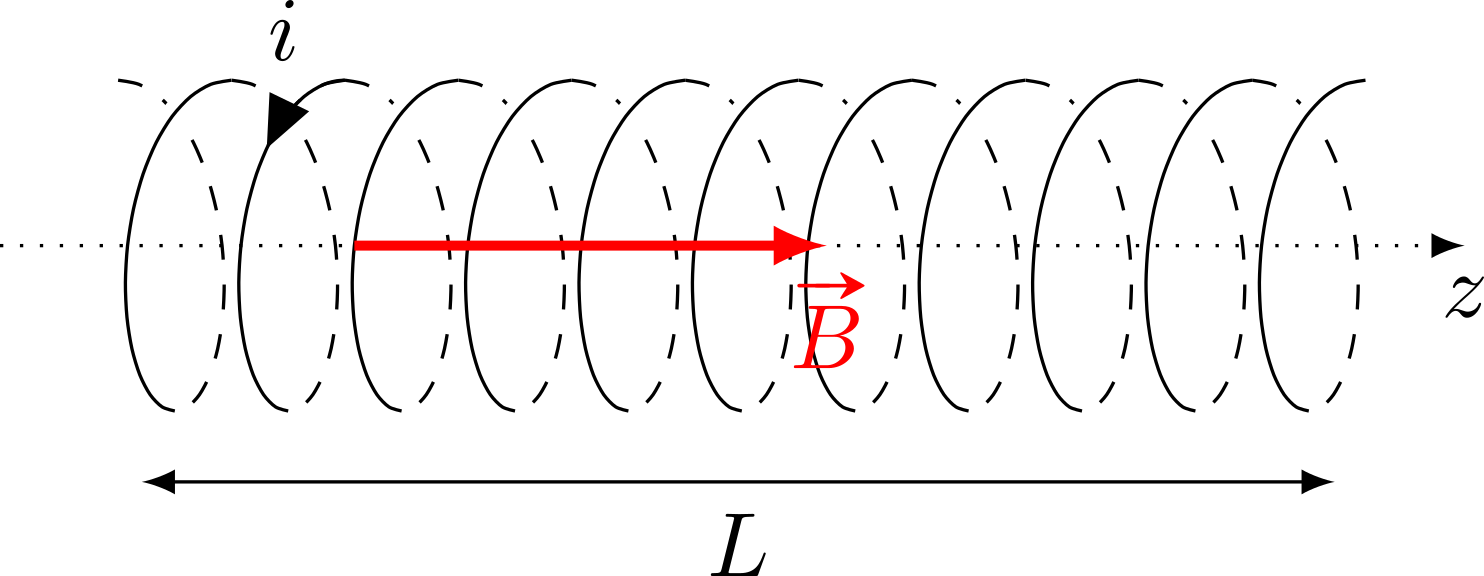
\includegraphics[width=\linewidth]{bobine_base}
		\captionsetup{justification=centering}
		\captionof{figure}{Bobine et champ magnétique}
		\label{fig:bobine}
	\end{center}
\end{minipage}
On le verra en électromagnétisme, le champ magnétique est \textbf{orienté
	par le courant}.

\begin{tcb*}(odgr)<lftt>'l'{Champs magnétiques}
	Le Tesla est une «~grande unité»~: il est très difficile de dépasser les
	\SI{10}{T}.
	\begin{itemize}[label=$\diamond$]
		\item À l'intérieur d'une bobine en TP, on a environ
		      \SI{e-4}{T}
		\item Une bobine avec $N = \num{1000}$, $L = \SI{10}{cm}$ et $i =
			      \SI{1}{A}$ donne \SI{e-2}{T}
		\item À la surface de la Terre, le champ magnétique est d'environ
		      \SI{5e-5}{T}
		\item Le champ magnétique au centre d'un IRM est d'environ
		      \SI{1}{T}
		\item Le champ magnétique d'un aimant permanent est d'environ
		      \SIrange{e-2}{e-1}{T}
	\end{itemize}
\end{tcb*}

\vspace{-12pt}
\section{La force de \textsc{Lorentz}}
On considèrera dans toute la suite des champs \textbf{uniformes}\footnote{Est
	uniforme une grandeur constante dans l'espace.} et
\textbf{stationnaires}\footnote{Est stationnaire une grandeur constante dans le
	temps.}.
\vspace{-12pt}

\subsection{Définition}
\begin{tcb*}(defi){Force de \textsc{Lorentz}}
	La force subie par une charge $q$ plongée dans un champ électrique $\Ef$ et
	un champ magnétique $\Bf$ est appelée \textbf{force de \textsc{Lorentz}},
	telle que
	\psw{
		\[\boxed{\Ff = q\left(\Ef + \vf \wedge \Bf\right)}\]
	}
	On appelle $\Ff_e = q\Ef$ la \textbf{force électrique} et $\Ff_m =
		q\vf\wedge\Bf$ la \textbf{force magnétique}
\end{tcb*}

\subsection{Comparaison au poids}

Les particules chargées sont généralement très légères et rapides~: pour un
électron, on a $m \approx \SI{e-30}{kg}$ et $\norm{\vf} \approx
	\SI{e6}{m.s^{-1}}$. Seulement, leur charge est également faible, avec $\abs{e}
	\approx \SI{e-19}{C}$ pour un électron ou un proton. Il est donc intéressant de
connaître la différence de force entre le poids qu'elle subit et la force de
\textsc{Lorentz}, ce qui nous permettrait de négliger le poids dans le PFD.
Avec $g \approx \SI{10}{m.s^{-2}}$, on trouve
\psw{
	\[\norm{\Pf} \approx \SI{e-29}{N}\]
}
Regardons ce qu'il en est pour les parties électrique et magnétique de la force
de \textsc{Lorentz}.
\bigbreak
\begin{itemize}[label=$\diamond$]
	\bitem{Partie électrique~:} $\norm{\Ff_e} = eE$, avec $E \approx \psw{
			\SI{e4}{V.m^{-1}}}$~:
	\[\norm{\Ff_e} \approx \psw{\SI{e-15}{N}}\]
	\vspace{-15pt}
	\bitem{Partie magnétique~:} $\norm{\Ff_m} = evB$, avec $B \approx
		\psw{\SI{e-2}{T}}$~:
	\[\norm{\Ff_m} \approx \psw{\SI{e-15}{N}}\]
	\vspace{-15pt}
\end{itemize}
\vspace{-15pt}
\begin{gather*}
	\beforetext{Ainsi, dans les deux cas, on a}
	\psw{
		\frac{\norm{\Ff_e}}{\norm{\Pf}} = \frac{\norm{\Ff_m}}{\norm{\Pf}} \approx
		\num{e14}
	}
\end{gather*}

\begin{tcb*}[cnt, bld](ror){Impact du poids vs. \textsc{Lorentz}}
	Pour des particules chargées dans des conditions générales, le poids est
	négligeable \textit{devant} la force de \textsc{Lorentz}.
\end{tcb*}

\subsection{Produit vectoriel}
Pour calculer la force magnétique, il va falloir manipuler les produits
vectoriels. Quelques rappels~:
\bigbreak
\begin{tcb*}(rapp){Produit vectoriel}
	Le produit vectoriel de deux vecteurs $\vv{u}$ et $\vf$ s'écrit
	$\vv{u}\wedge\vf$, et se lit «~u vectoriel v~». C'est un \textbf{vecteur}~:
	\smallbreak
	\noindent
	\begin{minipage}{0.70\linewidth}
		\begin{itemize}[label=$\diamond$]
			\item de direction \textbf{perpendiculaire} à $\vv{u}$ \textbf{et} à
			      $\vf$~:
			      \[
				      \psw{\vv{u}\wedge\vf \perp \vv{u}}
				      \qet
				      \psw{\vv{u}\wedge\vf \perp \vf}
			      \]
			\item de sens donné par la règle de la \textbf{main droite}~;
			\item de norme
			      $\quad \norm{\vv{u}\wedge\vf} =
				      \norm{\vv{u}}\norm{\vf}\abs{\sin(\tt)} \quad$
			      avec $\tt$ l'angle entre les deux vecteurs.
		\end{itemize}
	\end{minipage}
	\hfill
	\begin{minipage}{0.25\linewidth}
		\begin{center}
			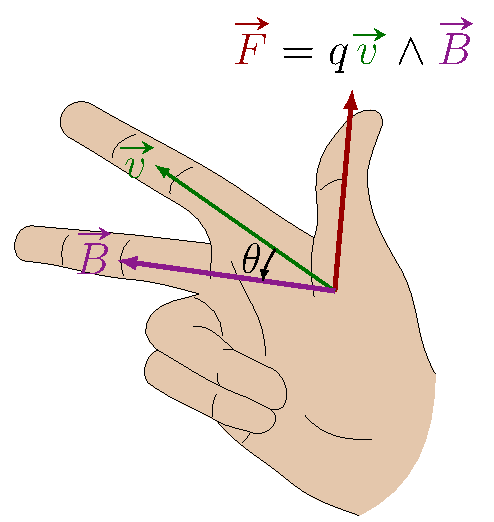
\includegraphics[width=.7\linewidth]{righthand_lorentz}
			\captionsetup{justification=centering}
			\captionof{figure}{Règle de la main droite}
			\label{fig:rhlorentz}
		\end{center}
	\end{minipage}
	\hfill
	~

	L'ordre des vecteurs est \textbf{primordial} dans un produit vectoriel~:
	c'est en effet un opérateur \textbf{antisymétrique}, c'est-à-dire qu'il
	respecte
	\[\boxed{\psw{\vv{u}\wedge\vf = -\vf\wedge\vv{u}}}\]
	Pour une base orthonormée \textbf{directe} (BOND), qu'elle soit cartésienne,
	cylindrique ou sphérique, le produit vectoriel de deux vecteurs de base
	donne le troisième avec un signe $+$ s'ils se suivent dans une permutation
	circulaire ($x\ra y\ra z \ra x$ ou $r\ra\tt\ra z\ra r$), et un signe $-$
	sinon. Par exemple~:
	\begin{gather*}
		\begin{aligned}
			\ux\wedge\uy & = \psw{\uz}  \\
			\uy\wedge\ux & = \psw{-\uz}
		\end{aligned}
		\qquad
		\begin{aligned}
			\uy\wedge\uz & = \psw{\ux}  \\
			\uz\wedge\uy & = \psw{-\ux}
		\end{aligned}
		\qquad
		\begin{aligned}
			\uz\wedge\ux & = \psw{\uy}  \\
			\ux\wedge\uz & = \psw{-\uy}
		\end{aligned}
	\end{gather*}
	Ces données permettent de calculer n'importe quel produit vectoriel exprimé
	dans une BOND. En termes de composantes des vecteurs, on pourra déterminer
	le produit vectoriel avec la «~règle du gamma~»~; par exemple~:
	% \begin{tikzpicture}
	% 	\node[below=4pt, gray, transform canvas={xshift=-5.5pt}]
	% 	(uxx) at (pic cs:uz) {$u_x$};
	% 	\tikzmark{uxx}{(uxx)}
	% \end{tikzpicture}
	% \begin{tikzpicture}
	% 	\node[below=4pt, gray, transform canvas={xshift=-5.5pt}]
	% 	(vxx) at (pic cs:vz) {$v_x$};
	% 	\tikzmark{vxx}{(vxx)}
	% \end{tikzpicture}
	% \tikz[remember picture, overlay]
	% \draw[-{Latex[length=2mm]}, orange!90!black, transform canvas={xshift=-5.5pt}]
	% (pic cs:ux) .. controls
	% (pic cs:vy) .. node[pos=.85, above right=-4pt and -1.5pt] {$\oplus$}
	% ($(pic cs:vy)!0.5!(pic cs:uy)$) .. controls
	% (pic cs:uy) .. node[pos=0.15, above left=-4pt and -1.5pt] {$\ominus$}
	% (pic cs:vx)
	% ;
	% \tikz[remember picture, overlay]
	% \draw[-{Latex[length=2mm]}, BlueViolet!70!black, transform canvas={xshift=-5.5pt}]
	% (pic cs:uy) .. controls
	% (pic cs:vz) .. node[pos=.85, above right=-4pt and -1.5pt] {$\oplus$}
	% ($(pic cs:vz)!0.5!(pic cs:uz)$) .. controls
	% (pic cs:uz) .. node[pos=0.15, above left=-4pt and -1.5pt] {$\ominus$}
	% (pic cs:vy)
	% ;
	% \tikz[remember picture, overlay]
	% \draw[-{Latex[length=2mm]}, ForestGreen, transform canvas={xshift=-5.5pt}]
	% (pic cs:uz) .. controls
	% (pic cs:vxx) .. node[pos=.85, above right=-4pt and -1.5pt] {$\oplus$}
	% ($(pic cs:vxx)!0.5!(pic cs:uxx)$) .. controls
	% (pic cs:uxx) .. node[pos=0.15, above left=-4pt and -1.5pt] {$\ominus$}
	% (pic cs:vz)
	% ;
	\[\vv{u}\wedge\vf
		= \mqty(u_x\tikzmark{ux}\\u_y\tikzmark{uy}\\u_z\tikzmark{uz})
		\wedge
		\mqty(v_x\tikzmark{vx}\\v_y\tikzmark{vy}\\v_z\tikzmark{vz})
		= \mqty(\color{BlueViolet!70!black}u_yv_z - u_zv_y\\\color{ForestGreen}u_zv_x -
		u_xv_z\\\color{orange!90!black}u_xv_y - u_yv_x)
	\]
	\vspace{12pt}
\end{tcb*}

\subsection{Puissance de la force de \textsc{Lorentz}}
\begin{tcb*}(prop){Puissance force magnétique}
	La puissance de la force de \textsc{Lorentz} est
	\psw{\[\Pc(\Ff) = q\Ef\cdot\vf\]}
	\textbf{La puissance de la force magnétique est nulle~: un champ magnétique ne
		peut pas accélérer ou ralentir une particule chargée mais ne peut que la
		dévier.}
\end{tcb*}
\begin{tcb*}(demo)<lftt>'l'{Puissance de \textsc{Lorentz}}
	La puissance de la force de \textsc{Lorentz} est~:
	\psw{
		\begin{align*}
			\Pc(\Ff)         & = \left(q\left(\Ef + \vf\wedge\Bf\right)\right)\cdot\vf
			\\\Lra
			\Pc(\Ff)         & = q\Ef\cdot\vf +
			q\underbracket[1pt]{\underbracket[1pt]{\vf\wedge\Bf}_{\perp\vf}\cdot\vf}_{=0}
			\\\Lra
			\Aboxed{\Pc(\Ff) & = q\Ef\cdot\vf}
			\qed
		\end{align*}
	}
	En effet, $\vf\wedge\Bf \perp \vf$, et le produit scalaire de deux vecteurs
	orthogonaux est nul. Ainsi, la partie magnétique de la force de \textsc{Lorentz}
	ne travaille pas~; le TPC donne alors
	\psw{\[\dv{\Ec_c}{t} = q\Ef\cdot\vf\]}
	c'est-à-dire que seule la \textbf{partie électrique} peut faire varier
	l'énergie cinétique, et donc la vitesse, d'une particule chargée.
	\hqed
\end{tcb*}

\subsection{Potentiel électrostatique}
\begin{tcb*}(prop){Force conservative et énergie potentielle}
	La force de \textsc{Lorentz} est \textbf{conservative}, et dérive d'une
	d'une énergie potentielle $\Ec_{p,e}$ telle que
	\psw{\[\Ec_{p,e} = -qEz\]}
	avec $E$ la norme du champ électrique subit et $z$ la position dans ce
	champ.
\end{tcb*}
\begin{tcb*}(demo)<lftt>'l'{Énergie potentielle}
	Le champ magnétique ne travaillant pas, on s'intéresse au travail
	élémentaire de la force électrique. Supposons un champ électrique $\Ef =
		E\uz$~:
	\psw{
		\begin{align*}
			\de W_{\ABr}(\Ff)         & = \Ff_e\cdot\dd\OM
			\\\Lra
			\de W_{\ABr}(\Ff)         & = qE\uz\cdot(\dd{x}\ux + \dd{y}\uy + \dd{z}\uz)
			\\\Lra
			\Aboxed{\de W_{\ABr}(\Ff) & = qE\dd{z}}
		\end{align*}
	}
	\psw{
		On a donc bien $\de W_{\ABr}(\Ff)$ qui ne \textbf{dépend pas du chemin
			suivi}~; elle est donc \textbf{conservative}, et on identifie $\Ec_{p,e}$ à
		partir de $\de W_{\ABr}(\Ff) = -\dd{\Ec_{p,e}}$, soit $\Ec_{p,e} = -qEz$.
	}
	\hqed
\end{tcb*}

\begin{tcb*}(rema)<lftt>'l'{Comparaison champ $\protect\Ef$ et champ
	$\protect\gf$}
	La situation avec un champ $\Ef$ est en essence tout à fait similaire à
	celle du poids, provenant d'un champ gravitationnel~: on obtient la même
	énergie potentielle à un signe près. En effet, la masse ne peut qu'être
	positive, alors qu'une charge peut être négative~; mais l'effet d'un champ
	$\Ef$ sur une particule chargée est en tous points similaire à celle de
	l'action de la gravité sur une masse $m$.
\end{tcb*}

Ainsi, puisque $\Ff_e$ est conservative, on a
\[\Ff_e = -\gd\Ec_{p,e}\]
Il est souvent utile de déterminer $\Ef$ plutôt que $\Ff$~; on introduit donc
une autre grandeur~:

\begin{tcb*}(defi){Potentiel électrostatique}
	Le \textbf{potentiel électrostatique} est la grandeur scalaire qui permet de
	calculer le champ $\Ef$ associé, tel que
	\psw{
		\[
			V = \frac{\Ec_{p,e}}{q}
			\Lra
			\boxed{\Ec_{p,e} = qV}
			\quad\Ra\quad
			\Ef = -\gd V
		\]
	}
\end{tcb*}

On retrouve alors les notions du début d'année en électrocinétique~:

\begin{tcb*}(defi){Tension}
	La \textbf{tension} entre deux points A et B est la \textbf{différence de
		potentiel} entre ces deux points~:
	\psw{
		\[\boxed{U_{\ABr} = V(\Ar) - V(\Br)}\]
	}
	\vspace{-15pt}
\end{tcb*}

On trouve finalement le lien entre champ électrique et tension entre deux
plaques chargées~: en utilisant
\[
	\Ec_{p,e} = -qEz
	\qet
	V = \Ec_{p,e}/q \Lra V = -Ez
	\qet
	U_{\ABr} = V(\Ar) - V(\Br)
\]
on a
\psw{\[U_{\ABr} = -Ez_\Ar + Ez_\Br = E(z_\Br - z_\Ar) = Ed\]}
\vspace{-15pt}
\begin{tcb*}(ror){Tension et et champ électrique}
	En appliquant une tension $U$ entre deux grilles planes parallèles et
	distantes de $d$, on obtient un champ électrique \textbf{perpendiculaire}
	aux grilles, dirigé vers les potentiels \textbf{décroissants} (borne
	$\ominus$) de norme
	\psw{
		\[\norm{\Ef} = \frac{U}{d}\]
	}
\end{tcb*}

Voilà donc comment faire un condensateur~! Mais alors, à quoi ça sert~?

\section{Mouvement dans un champ électrique}
\subsection{Situation générale}\label{ssec:egen}
\begin{enumerate}[label=\sqenumi]
	\begin{minipage}[t]{0.70\linewidth}
		\bitem{Système~:} \{particule\} de masse $m$ de charge $q$ dans un champ
		$\Ef$.
		\bitem{Schéma~:} ci-contre.
		\bitem{Modélisation~:}
		\begin{itemize}[label=$\diamond$, leftmargin=10pt]
			\item Repère~: cartésien, $\uz$ $\perp$ grilles,
			      soit $\Ef = E\uz$ avec $E = U/d$
			\item Instant initial~: la particule part de $z=0$, $\OM(0) = \of$
		\end{itemize}
		\bitem{BDF~:}
		\psw{
			\[
				\begin{array}{ll}
					\textbf{Poids}            & \text{négligeable \textbf{devant }}\Ff \\
					\textbf{Force électrique} & \Ff = q\Ef = qE\uz
				\end{array}
			\]
		}
	\end{minipage}
	\hfill
	\begin{minipage}[t]{0.28\linewidth}
		~
		\begin{center}
			\sswitch{
				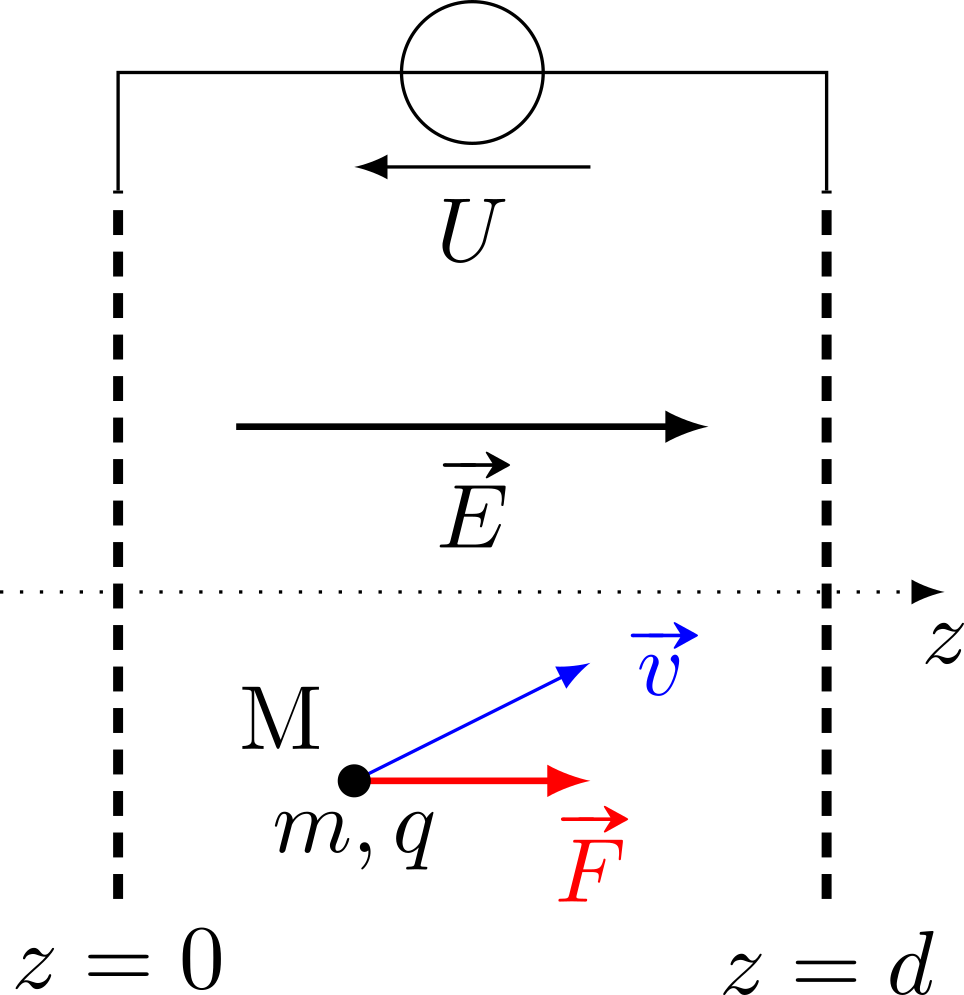
\includegraphics[width=.8\linewidth, draft=true]{chp_E-base}
			}{
				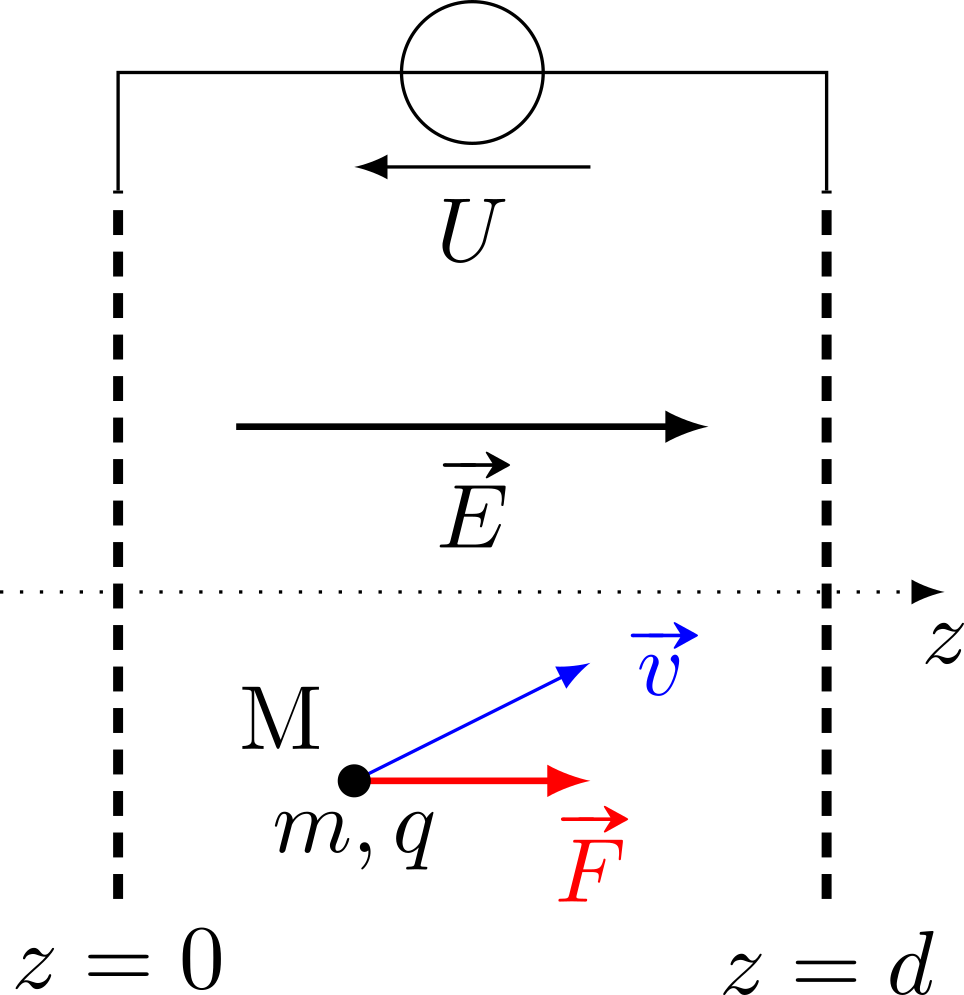
\includegraphics[width=.8\linewidth]{chp_E-base}
			}
			\vspace{-15pt}
			\captionof{figure}{Situation générale}
			\label{fig:chp_E_base}
		\end{center}
	\end{minipage}
\end{enumerate}
\begin{enumerate}[label=\sqenumi, resume]
	\bitem{PFD~:}
	\vspace{-18pt}
	\psw{
		\[m\af = \Ff\]
	}
	\vspace{-15pt}
	\bitem{Équations scalaires~:}
	\psw{
		\begin{empheq}[left=\empheqlbrace]{align*}
			m\xpp &= 0\\
			m\ypp &= 0\\
			m\zpp &= qE
		\end{empheq}
	}
	\bitem{Réponse aux questions.} Il est possible d'intégrer ces équations pour
	obtenir les équations horaires, $E$ étant uniforme et stationnaire~; on
	va distinguer deux cas selon la vitesse initiale de la particule.
\end{enumerate}

\subsection{Accélération d'une particule chargée}
On suppose ici une particule chargée positivement ($q > 0$), arrivant en $z = 0$
avec une vitesse $\vfo = v_0\uz$, c'est-à-dire \textbf{dans le sens du champ}.
On s'intéresse à sa vitesse en sortie, en $z=d$. Comme le système est
\textbf{conservatif} et qu'on s'intéresse à un instant précis du mouvement, il
est plus astucieux d'utiliser le \textbf{TEM} plutôt que le PFD~: \bigbreak
\begin{itemize}[label=$\diamond$]
	\bitem{En $z=0$~:} la norme de la vitesse est $v_0$, et l'énergie potentielle
	est $qV(0)$, d'où l'énergie mécanique
	\psw{\[\Ec_m(0) = \frac{1}{2}mv_0{}^2 + qV(0)\]}
	\vspace{-15pt}
	\bitem{En $z=d$~:} la norme de la vitesse est $v_f$, et l'énergie potentielle
	est $qV(d)$, d'où l'énergie mécanique
	\psw{\[\Ec_m(d) = \frac{1}{2}mv_f{}^2 + qV(d)\]}
	\vspace{-15pt}
\end{itemize}
Ainsi
\vspace{-18pt}
\psw{
	\begin{align*}
		\frac{1}{2}mv_0{}^2 + qV(0) & = \frac{1}{2}mv_f{}^2 + qV(d)
		\\\Lra
		v_f{}^2                     & = v_0{}^2 + \frac{2q}{m}\left(V(0) - V(d)\right)
		\\\Lra
		\Aboxed{v_f                 & = \sqrt{v_0{}^2 + \frac{2qU}{m}}}
	\end{align*}
}

\begin{tcb*}[cnt, bld](ror){Particule $\protect\vfo \parr \protect\Ef$}
	Une particule chargée positivement et lancée dans le sens d'un champ
	électrique est accélérée, sa vitesse finale augmentant en $\sqrt{U}$.
\end{tcb*}

En faisant l'application numérique pour un proton de charge $e =
	\SI{1.602e-19}{C}$, de masse $m = \SI{1.673e-27}{kg}$ partant de $v_0 =
	\SI{0}{m.s^{-1}}$ et accéléré par $U = \SI{1}{kV}$, on trouve
\[v_f = \SI{4.4e5}{m.s^{-1}} = \SI{440}{km.s^{-1}}\]

\begin{tcb*}(rema)<lftt>'l'{Accélération rectiligne}
	\begin{itemize}
		\item L'électron-volt est une unité d'énergie, telle que
		      \[\SI{1.602e-19}{J} = \SI{1.602e-19}{C}\times\SI{1}{V} =
			      e\times\SI{1}{V}\]
		      C'est l'énergie cinétique que gagne un électron (ou un proton)
		      lorsqu'il est accéléré par une tension de \SI{1}{V}. Dans les
		      accélérateurs de particules modernes, on touche au \si{TeV}
		      (tera-électron-volt)
		\item Si $U<0$ ou $q<0$, on peut ralentir la particule chargée. Elle
		      peut même faire demi-tour si l'énergie potentielle acquise est
		      supérieure à son énergie cinétique initiale~; elle ressortira alors
		      avec la même énergie cinétique qu'au départ (puisque
		      $\Ec_{p,e}(z=0)$ ne change pas), donc la même vitesse en norme, mais
		      bien sûr de sens opposé.
	\end{itemize}
\end{tcb*}

\subsection{Déviation d'une particule chargée}
\noindent
\begin{minipage}[t]{.60\linewidth}
	On considère cette fois une particule chargée arrivant
	\textbf{perpendiculairement} à un champ $\Ef$. Prenons $\vfo = v_0\ux$ et $\Ef =
		E\uz$, avec $E=U/d$.  On reprend le résultat obtenu dans la situation générale
	(\ref{ssec:egen})~:
	\begin{empheq}[left=\empheqlbrace]{align*}
		m\xpp &= 0\\
		m\ypp &= 0\\
		m\zpp &= qE
	\end{empheq}
	On intègre, avec $\xp(0) = v_0$ et $\zp(0) = 0$~; on ignore le mouvement en
	$y$~; on intègre une seconde fois, avec $x(0) = 0 = z(0)$~:
\end{minipage}
\hfill
\begin{minipage}[t]{.39\linewidth}
	\vspace{0pt}
	\begin{center}
		\sswitch{
			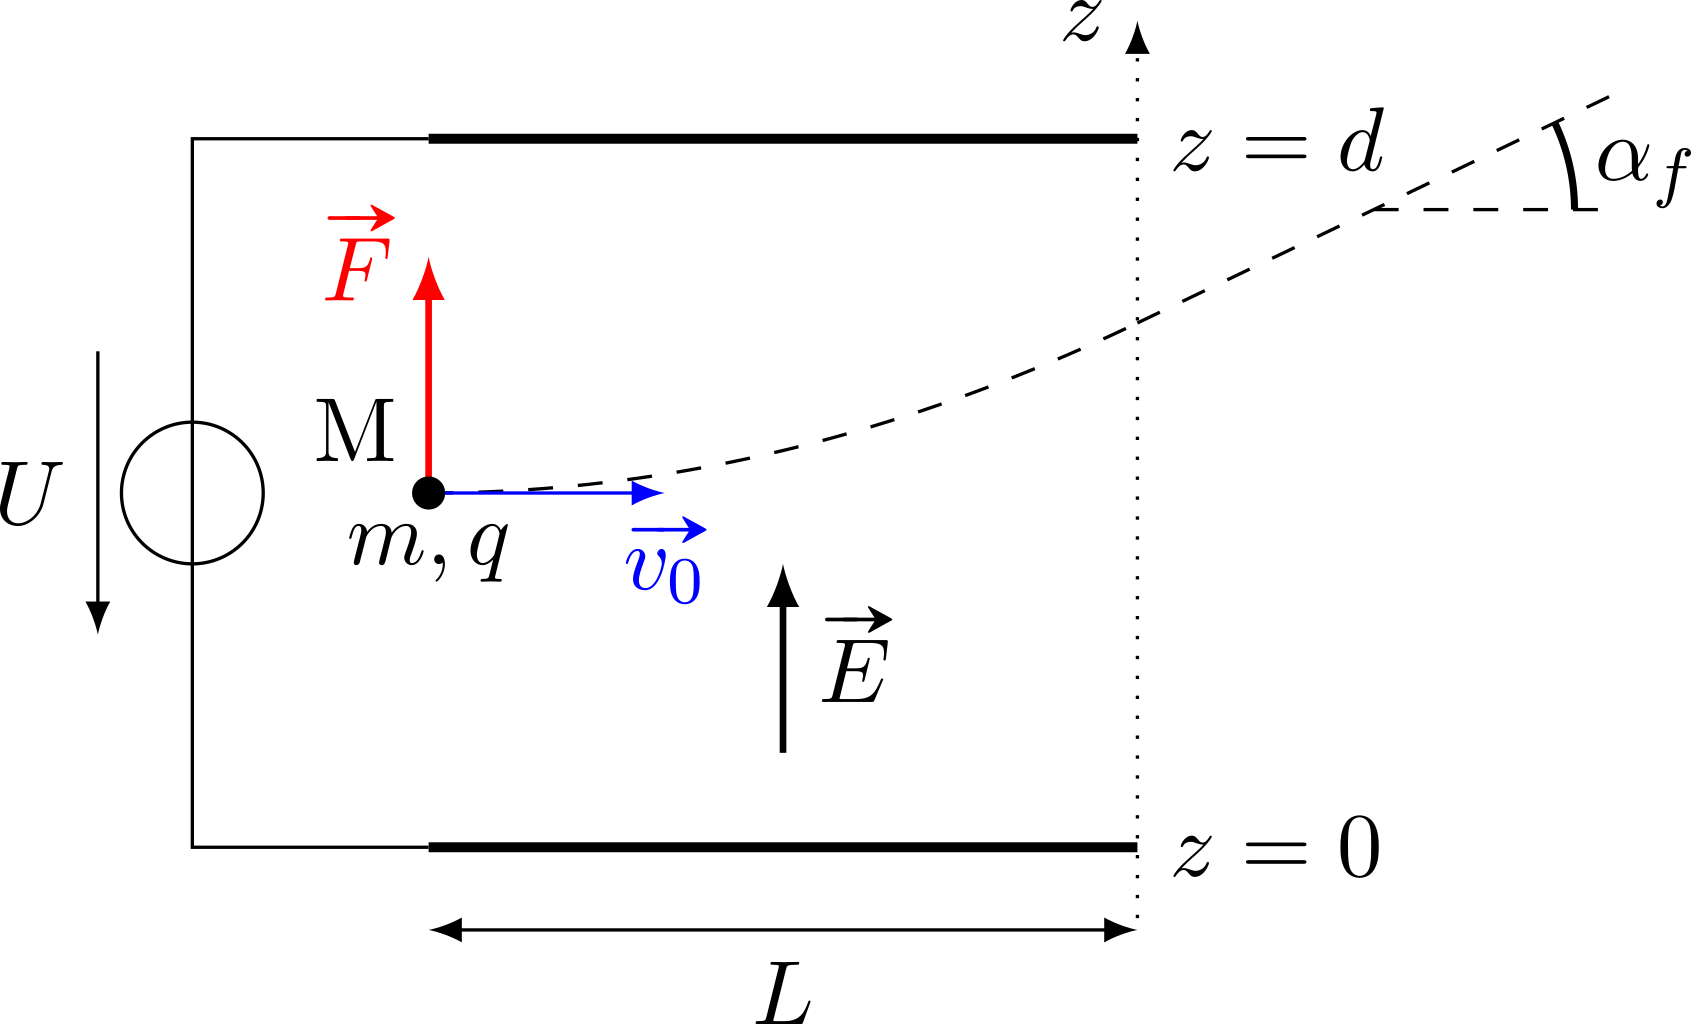
\includegraphics[width=\linewidth, draft=true]{chp_E-dev}
		}{
			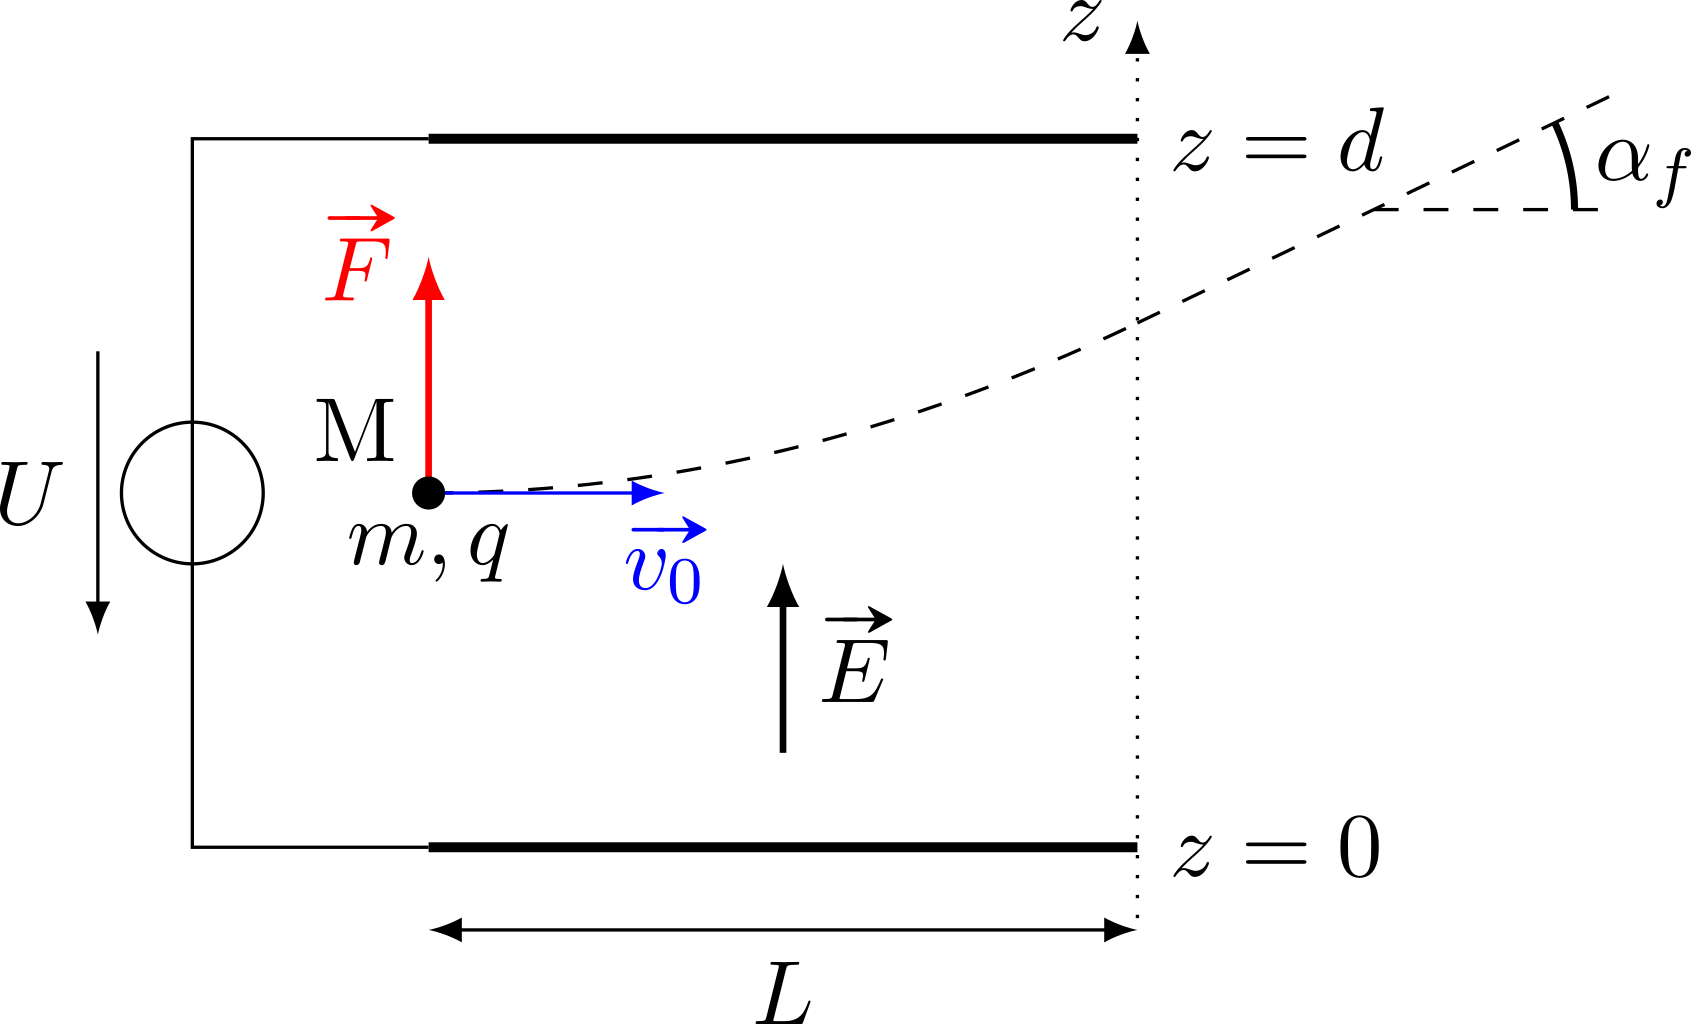
\includegraphics[width=\linewidth]{chp_E-dev}
		}
		\vspace{-15pt}
		\captionof{figure}{Situation de déviation}
		\label{fig:edev}
	\end{center}
\end{minipage}

\begin{gather*}
	\psw{
		\left\{
		\begin{aligned}
			\xp & = v_0           \\
			\zp & = \frac{qE}{m}t
		\end{aligned}
		\right.
	}
	\Lra
	\psw{
		\left\{
		\begin{aligned}
			x(t) & = v_0t             \\
			z(t) & = \frac{qE}{2m}t^2
		\end{aligned}
		\right.
	}
\end{gather*}
On trouve alors l'équation de la trajectoire~:
\psw{\[\boxed{z(x) = \frac{qE}{2mv_0{}^2}x^2}\]}
C'est une trajectoire parabolique, en tout point \textbf{similaire à la
	chute libre}.

\begin{tcb*}(appl)<lftt>'l'{Angle de déviation}
	On peut déterminer l'angle de déviation $\a_f$ entre la trajectoire de la
	particule au départ de son mouvement, et une fois qu'elle a quitté le champ
	$\Ef$. On trouve le temps de sortie $t_f$ tel que $x(t_f) = L$, soit $t_f =
		L/v_0$.
	\bigbreak
	On trouve l'angle de sortie en prenant
	\[
		\psw{\tan\a_f = \dv{z}{x} = \frac{\zp(t_f)}{\xp(t_f)}}
		\qor
		\left\{
		\begin{aligned}
			\xp(t_f) & = v_0              \\
			\zp(t_f) & = \frac{qEL}{mv_0}
		\end{aligned}
		\right.
	\]
	Avec $E = U/d$, et si l'angle est petit, on a donc
	\[\tan\a_f \approx \psw{\boxed{\a_f = \frac{qUL}{mdv_0{}^2}}}\]
	Ainsi, l'angle de déviation \textbf{est proportionnel à $U$}.
\end{tcb*}

\begin{tcb*}[cnt, bld](ror){Particule $\protect\vfo \perp \protect\Ef$}
	Une particule chargée positivement et lancée dans le sens d'un champ
	électrique est déviée, son angle final est proportionnel à $U$.
\end{tcb*}

\subsection{Applications}
On utilise rarement le champ $\Ef$ seul, il est souvent utilisé avec $\Bf$. On
peut néanmoins citer quelques applications~:
\begin{itemize}[label=$\diamond$]
	\bitem{Accélérateur linéaire.} On peut accélérer une particule chargée grâce
	à un champ électrique.
	\bitem{Oscilloscope analogique.} Un faisceau d'électrons de vitesse initiale
	fixée (grâce à un accélérateur linéaire) est dévié par la tension de
	mesure. Cette déviation est proportionnelle à la tension mesurée. En
	utilisant un écran fluorescent, on visualise l'impact des électrons et
	ainsi la tension mesurée en balayant l'écran à une vitesse déterminée
	par le calibre temporel.
\end{itemize}

\section{Mouvement dans un champ magnétique}
\subsection{Mise en équation}
\begin{enumerate}[label=\sqenumi]
	\bitem{Système~:} \{particule\} de masse $m$ de charge $q$ dans un champ
	$\Bf$.
	\bitem{Schéma~:}
	\begin{center}
		\sswitch{
			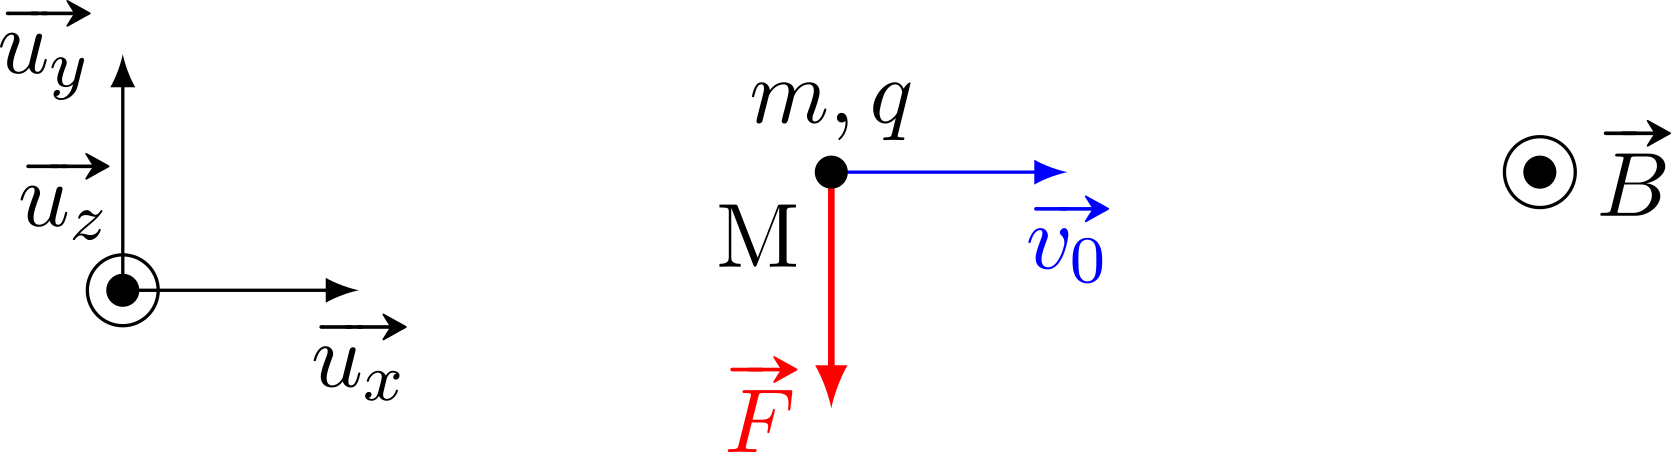
\includegraphics[scale=1, draft=true]{chp_B-base}
		}{
			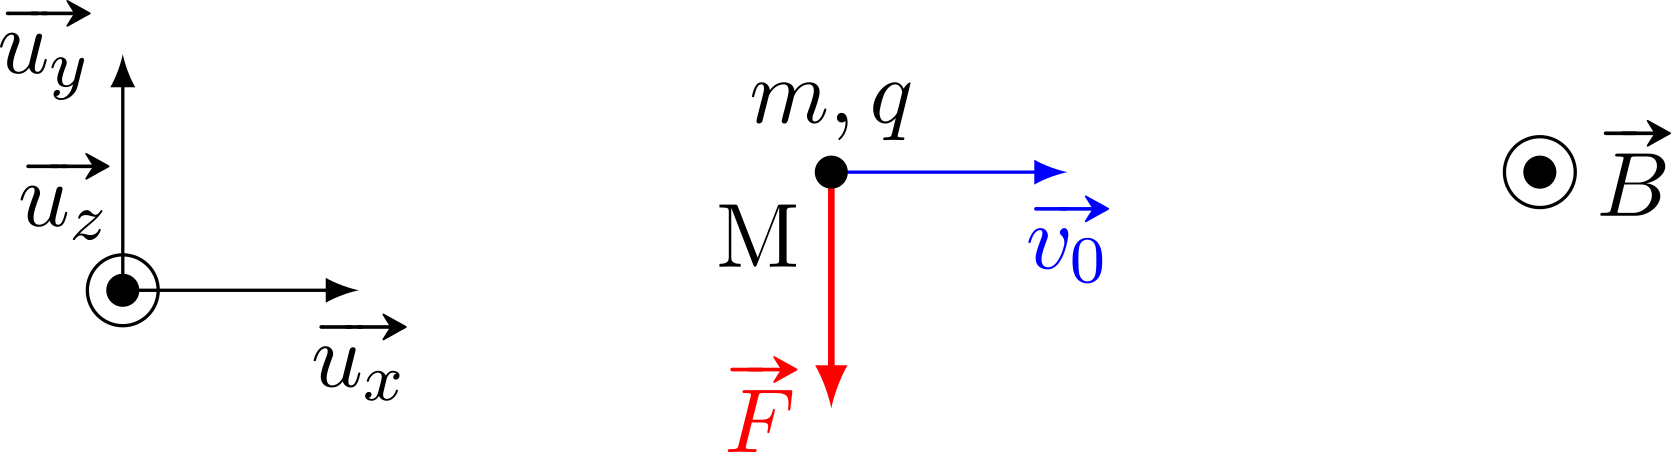
\includegraphics[scale=1]{chp_B-base}
		}
		% \vspace{-15pt}
		\captionof{figure}{Situation initiale}
		\label{fig:chp_B_base}
	\end{center}
	\bitem{Modélisation~:}
	\begin{itemize}[label=$\diamond$, leftmargin=10pt]
		\item Repère~: cartésien, $\uz$ direction de $\Bf$
		      soit $\Bf = B\uz$
		\item Instant initial~: la particule part de l'origine, $\OM(0) =
			      \of$
	\end{itemize}
	\bitem{BDF~:}
	\psw{
		\[
			\begin{array}{ll}
				\textbf{Poids}            & \text{négligeable \textbf{devant }}\Ff \\
				\textbf{Force magnétique} & \Ff = q\vf\wedge\Bf =
				\mqty(q\xp                                                         \\q\yp\\q\zp)\wedge\mqty(0\\0\\B)\\
				\Lra                      & \Ff = q\yp B\ux -q\xp B\uy
			\end{array}
		\]
	}
	\bitem{PFD~:}
	\[m\af = \Ff\]
	\bitem{Équations scalaires~:}
	\psw{
		\begin{empheq}[left=\empheqlbrace]{align*}
			m\xpp &= q\yp(t)B\\
			m\ypp &= -q\xp(t)B\\
			m\zpp &= 0
		\end{empheq}
	}
	\bitem{Réponse aux questions.} Ici aussi, on va distinguer deux cas selon la
	colinéarité de la vitesse initiale avec le champ.
\end{enumerate}

On remarque cependant, avant toute évolution due aux conditions initiales, que
le TPC nous donne une information sur le futur du système. En effet, la force
magnétique ne travaillant pas ($\vf\wedge\Bf \perp \vf$), on a
\[\dv{\Ec_c}{t} = 0\]
donc la vitesse est constante en norme, c'est-à-dire que le mouvement est
uniforme, et notamment
\[v_x(t)^2 + v_y(t)^2 + v_z(t)^2 = \cte\]
Or, avec la projection du PFD on a $\zpp = 0 \Ra \zp = \cte$, donc on sait déjà
que
\begin{tcb*}[cnt](ror){Analyse du mouvement en champ $\protect\Bf$}
	Le mouvement dans un champ $\Bf$ dirigé selon $\uz$ est \textbf{uniforme},
	et tel que
	\[\boxed{v_x(t)^2 + v_y(t)^2 = \cte}\]
\end{tcb*}
Étudions les deux cas intéressants.

\subsection{Vitesse initiale colinéaire au champ}
Prenons $\vf(0) = v_0\uz$. Comme $v_x(t)^2 + v_y(t)^2$ et qu'on part avec une
vitesse nulle sur $\ux$ et $\uy$, alors $v_x(t)$ et $v_y(t)$ sont nulles à tout
instant. La composante de $v_z(t)$ est quant à elle également constante, et
égale à $v_0$. Ainsi,
\begin{tcb*}[cnt](ror){Particule avec $\protect\vfo \parr \protect\Bf$}
	Une particule chargée de vitesse initiale colinéaire au champ magnétique a
	un mouvement rectiligne uniforme.
\end{tcb*}

Regardons l'autre situation.
\subsection{Vitesse initiale perpendiculaire au champ}
Prenons
\[\vf(0) = v_0\ux\]
$v_z(t)$ étant constant et $v_z(0)$ étant nulle, il n'y a pas de mouvement en
$z$~: le mouvement est donc \textbf{plan}.

\subsubsection{Trajectoire}
Avec le PFD précédent~:
\begin{gather*}
	\psw{
		\left\{
		\begin{aligned}
			\xpp(t) & = \frac{qB}{m}\yp(t)  \\
			\ypp(t) & = -\frac{qB}{m}\xp(t)
		\end{aligned}
		\right.
	}
	\Ra
	\psw{
		\left\{
		\begin{aligned}
			\xp(t) & = \frac{qB}{m}y(t) + v_0 \\
			\yp(t) & = -\frac{qB}{m}x(t) + 0
		\end{aligned}
		\right.
	}
\end{gather*}
Étant donné que $v_x(t)^2 + v_y(t)^2 = \cte = v_0{}^2$, on a
\psw{
\[
	\left(\frac{qB}{m}y(t) + v_0\right)^2 + \left(-\frac{qB}{m}x(t)\right)^2 =
	v_0{}^2
\]
}
soit, en notant $\w_c = \abs{q}B/m$~:
\psw{
	\[
		\left(y + \frac{mv_0}{qB}\right)^2 + (x)^2 = \left( \frac{v_0}{\w_c}
		\right)^2
	\]
}
On reconnaît l'équation d'un cercle en coordonnées cartésiennes~:
\begin{tcb*}(rapp){Équation cartésienne d'un cercle}
	L'équation cartésienne d'un cercle de centre $(x_0,y_0)$ et de rayon $R$
	est~:
	\[(x-x_0)^2 + (y-y_0)^2 = R^2\]
\end{tcb*}
Dans notre cas, le centre est $\DS\left(0,-\frac{mv_0}{qB}\right)$ et le rayon
est $\DS R_c = \frac{v_0}{\w_c} = \frac{v_0m}{\abs{q}B}$
\begin{itemize}[label=$\diamond$]
	\item Si $q>0$, alors $q = \abs{q}$ et le centre est en
	      $\DS\left(0,-\frac{v_0}{\w_c}\right) = (0,-R_c)$~;
	\item Si $q>0$, alors $q = -\abs{q}$ et le centre est en
	      $\DS\left(0,\frac{v_0}{\w_c}\right) = (0,R_c)$~;
\end{itemize}
On introduit alors le vocabulaire suivant~:
\begin{tcb*}(defi){Mouvement circulaire en champ $\protect\Bf$}
	Les constantes $R_c$ et $\w_c$ sont appelées \textbf{rayon cyclotron} et
	\textbf{pulsation cyclotron}, et sont telles que
	\[
		R_c = \frac{v_0}{\w_c}
		\qet
		\w_c = \frac{\abs{q}B}{m}
	\]
\end{tcb*}

\begin{minipage}{0.45\linewidth}
	\begin{center}
		\sswitch{
			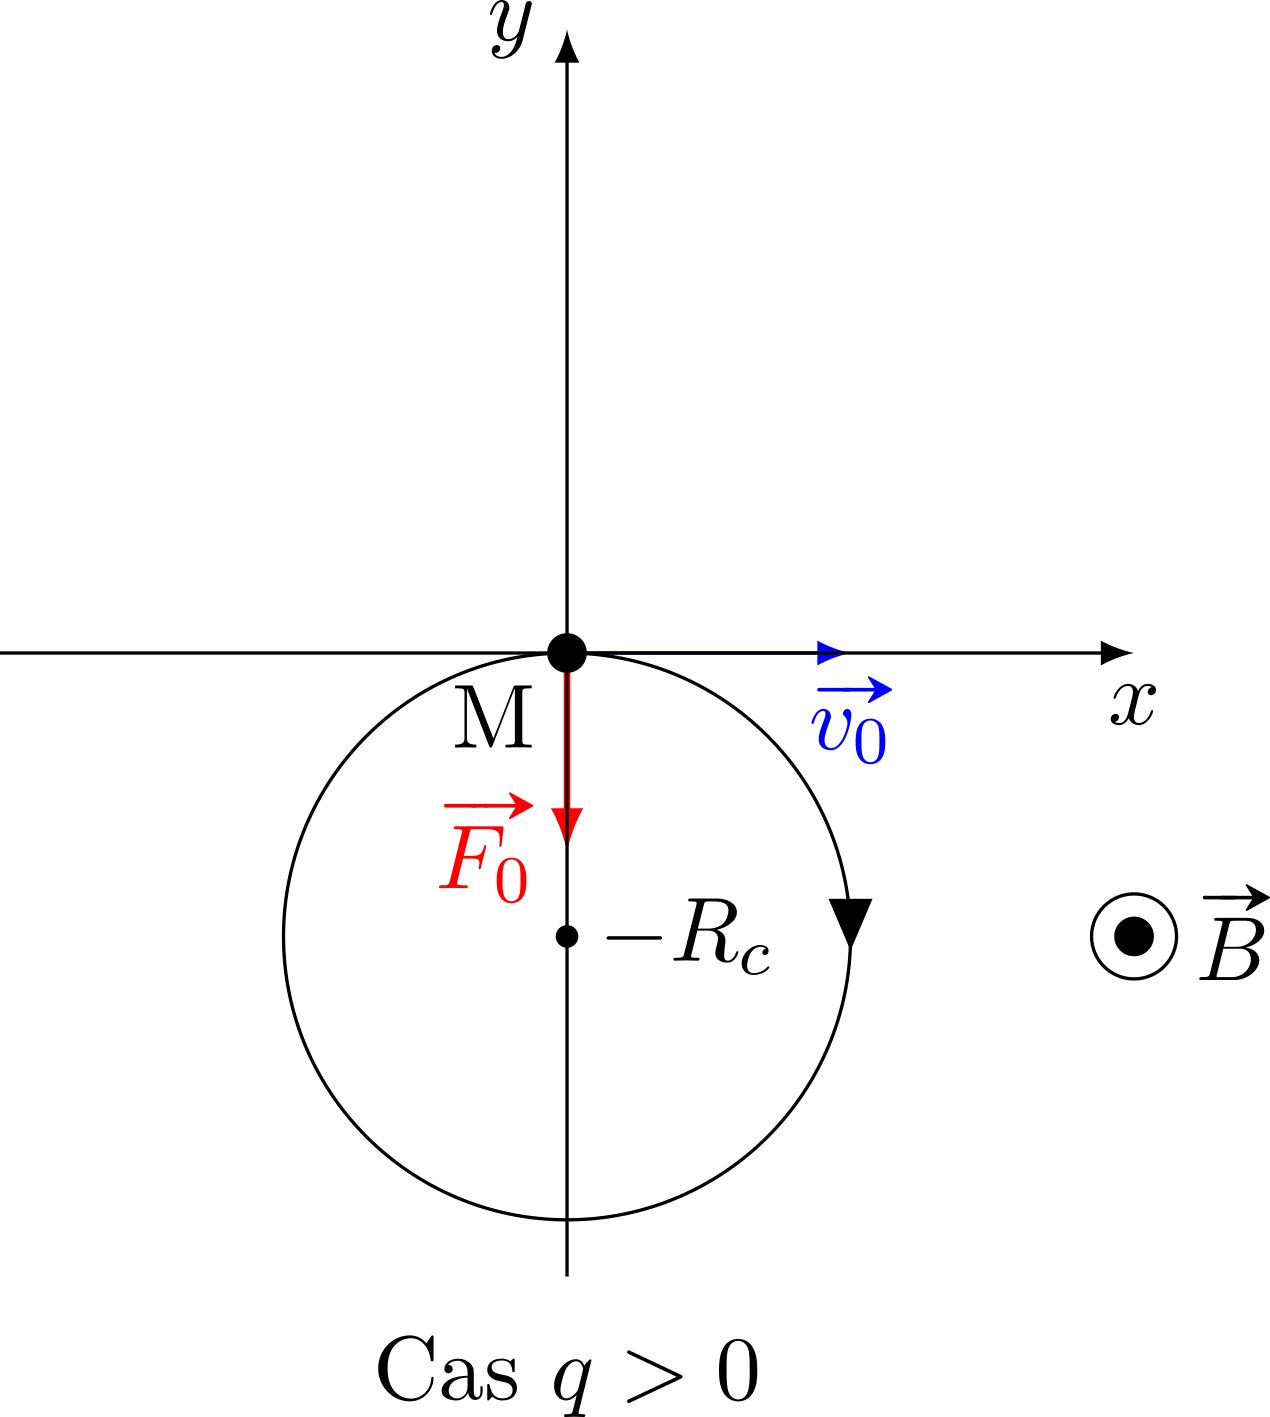
\includegraphics[width=5cm, draft=true]{chp_B-cercleqpos}
		}{
			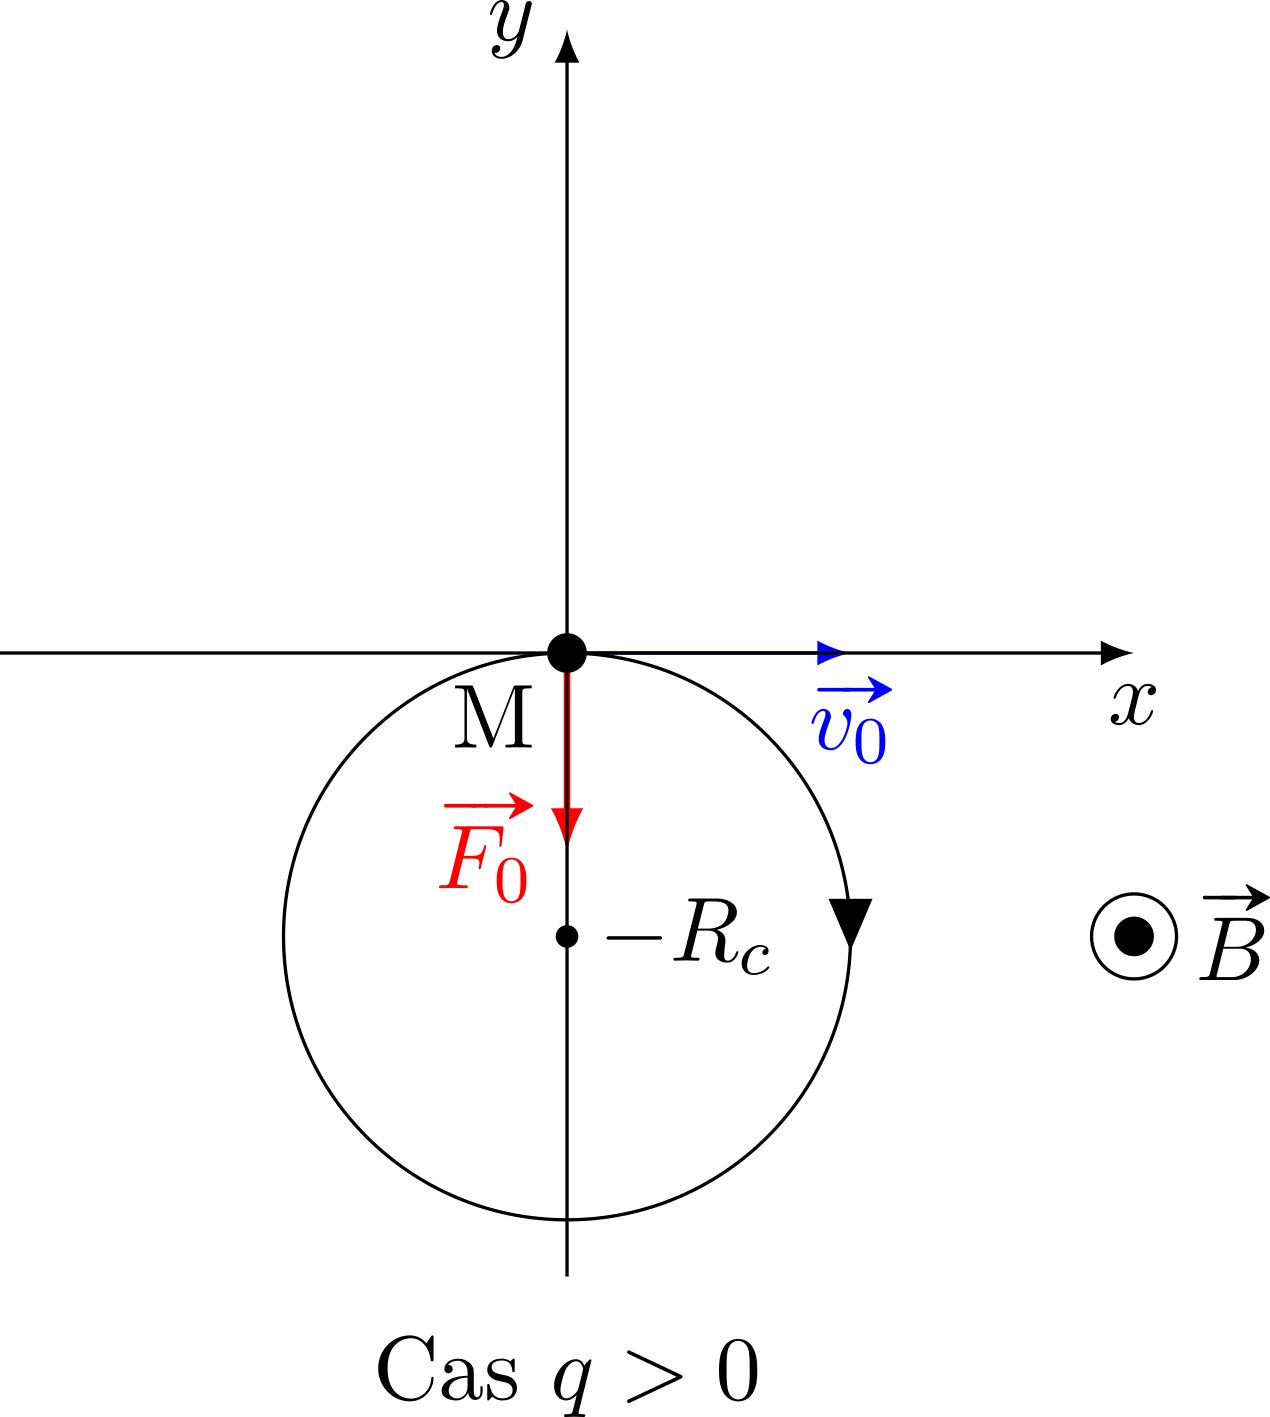
\includegraphics[width=5cm]{chp_B-cercleqpos}
		}
		\vspace{-15pt}
		\captionof{figure}{Cas $q>0$}
		\label{}
	\end{center}
\end{minipage}
\hfill
\begin{minipage}{0.45\linewidth}
	\begin{center}
		\sswitch{
			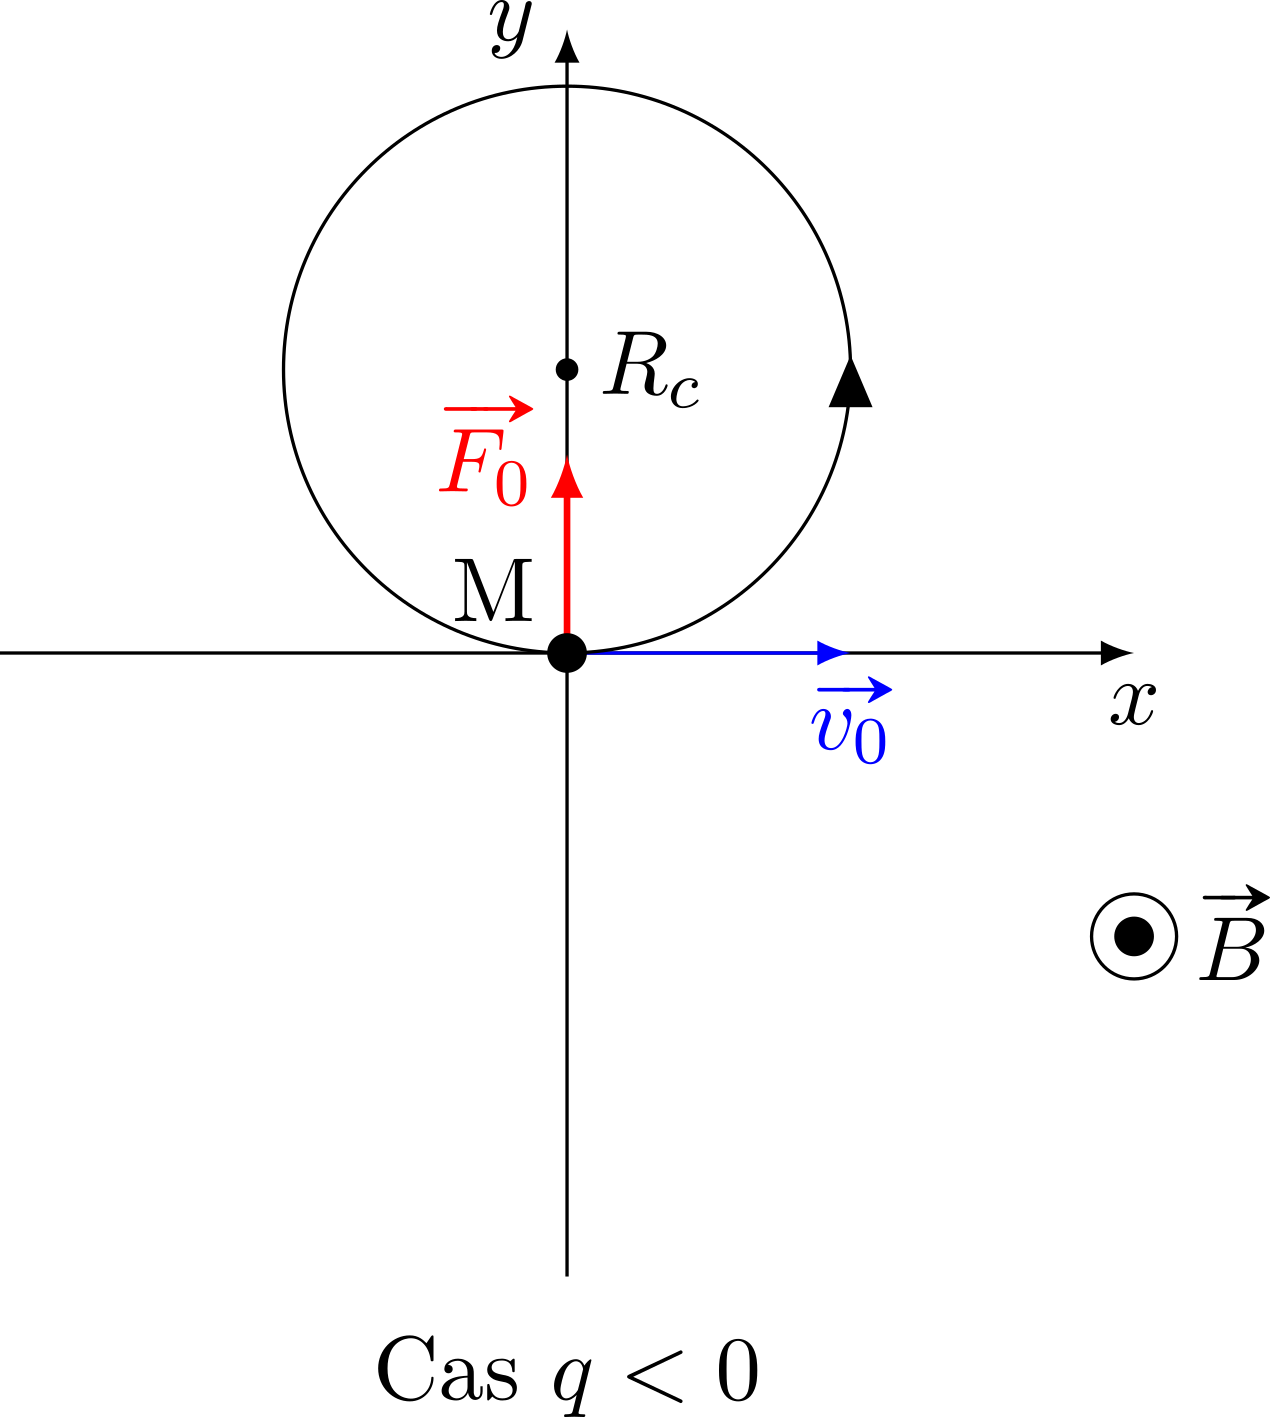
\includegraphics[width=5cm, draft=true]{chp_B-cercleqneg}
		}{
			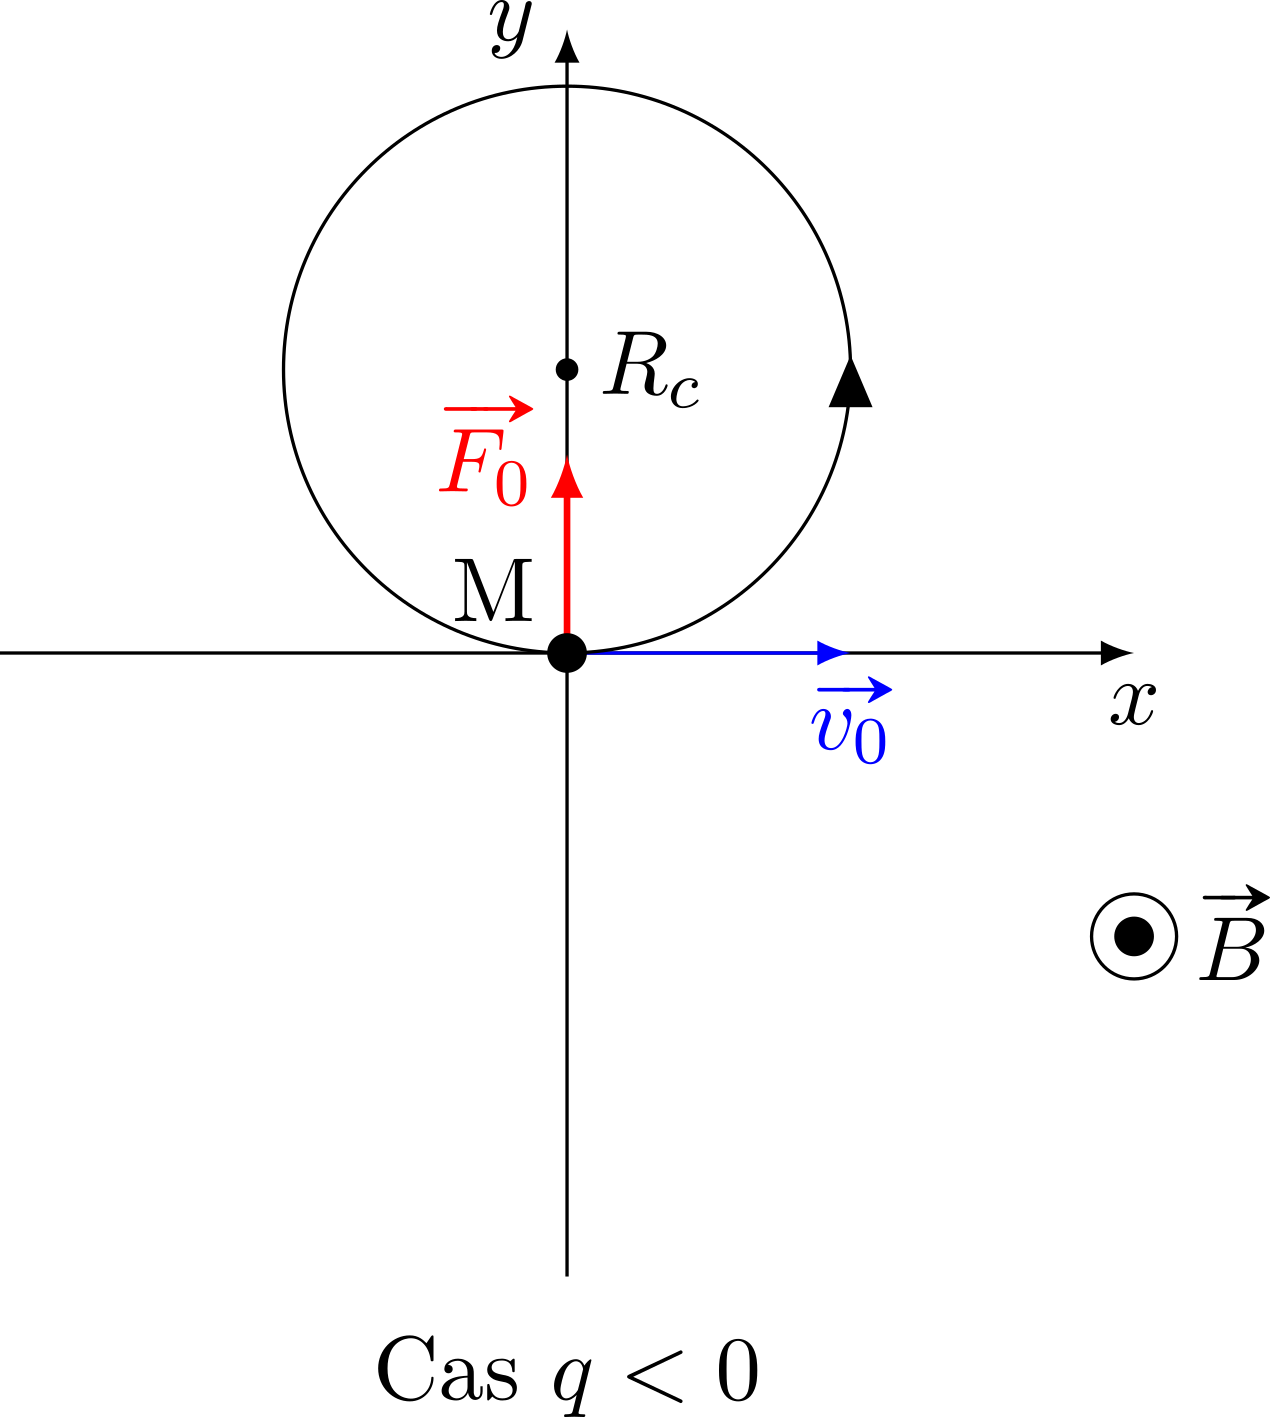
\includegraphics[width=5cm]{chp_B-cercleqneg}
		}
		\vspace{-15pt}
		\captionof{figure}{Cas $q<0$}
		\label{}
	\end{center}
\end{minipage}

\subsubsection{Équations horaires}
\begin{itemize}[label=$\diamond$]
	\bitem{Sur $x$~:} On part de $\yp = -qBx/m$ que l'on injecte dans la
	projection sur $\ux$ du PFD~:
	\psw{
		\begin{gather*}
			\xpp(t) = \frac{qB}{m}\yp(t) = - \left( \frac{qB}{m} \right)^2x(t)
			\\\Lra
			\boxed{\xpp(t) + \w_c{}^2x(t) = 0}
		\end{gather*}
	}
	On a donc la solution générale
	\psw{
		\begin{gather*}
			x(t) = A\cos(\w_ct) + B\sin(\w_ct)
		\end{gather*}
	}
	Et avec les conditions initiales
	\begin{gather*}
		x(0) = A
		\qor
		x(0) = 0
		\qdonc
		A = 0
		\\
		\xp(0) = \w_cB
		\qor
		\xp(0) = v_0
		\qdonc
		B = \frac{v_0}{\w_c}
		\\\Ra
		\psw{\boxed{x(t) = \frac{v_0}{\w_c}\sin(\w_ct)}}
	\end{gather*}
	\bitem{Sur $y$~:} On part de $\xp = qBy/m + v_0$ que l'on injecte dans la
	projection sur $\uy$ du PFD~:
	\psw{
		\begin{gather*}
			\ypp(t) = -\frac{qB}{m}\xp(t) = - \left( \frac{qB}{m} \right)^2y(t)
			- \frac{qB}{mv_0}
			\\\Lra
			\boxed{\ypp(t) + \w_c{}^2y(t) = -\w_c{}^2\frac{mv_0}{qB}}
		\end{gather*}
	}
	On a donc la solution générale
	\psw{
		\begin{gather*}
			y(t) = A\cos(\w_ct) + B\sin(\w_ct) - \frac{mv_0}{qB}
		\end{gather*}
	}
	Et avec les conditions initiales
	\begin{gather*}
		y(0) = A - \frac{mv_0}{qB}
		\qor
		y(0) = 0
		\qdonc
		A = \frac{mv_0}{qB}
		\\
		\yp(0) = \w_cB
		\qor
		\yp(0) = 0
		\qdonc
		B = 0
		\\\Ra
		\psw{\boxed{y(t) = \frac{mv_0}{qB}(\cos(\w_ct)-1)}}
	\end{gather*}
\end{itemize}
\begin{tcb*}[cnt, bld](ror){Particule avec $\protect\vfo \perp \protect\Bf$}
	Lors du mouvement d'une particule chargée dans un champ $\Bf$
	perpendiculaire à sa vitesse initiale $v_0$, la particule décrit un cercle de
	rayon $R_c$, de centre $(0,\pm R_c)$ à la vitesse angulaire $\w_c$.
\end{tcb*}

\subsection{Cas général}
Supposons $\vfo = v_{0,x}\ux + v_{0,z}\uz$. Les équations du mouvement
découplent le mouvement dans le plan $xy$ et selon $z$~:
\begin{itemize}
	\item Sur $z$ on garde une vitesse constante~: $v_z(t) = v_{0,z}$~;
	\item Pour les composantes sur $x$ et $y$, on a $v_x(t)^2 + v_y(t)^2 =
		      v_{0,x}{}^2$ et les mêmes équations différentielles~: le mouvement est
	      un cercle de rayon $R = \frac{v_{0,x}}{\w_c}$.
\end{itemize}
Ainsi, la trajectoire est la superposition d'une rotation circulaire uniforme
autour de $(\Or z)$ et d'une translation le long de cet axe~: c'est un
\textbf{mouvement hélicoïdal}. Une animation est disponible en
ligne\footnote{\url{https://phyanim.sciences.univ-nantes.fr/Meca/Charges/general.php}}.

\subsection{Applications}
\begin{itemize}[label=$\diamond$]
	\bitem{Spectromètre de masse.} Un spectromètre de masse permet de
	\textbf{mesurer la masse d'atomes}, et éventuellement de déterminer les
	abondances isotopiques (utilisable par exemple pour la datation). Le
	principe est le suivant~:
	\begin{center}
		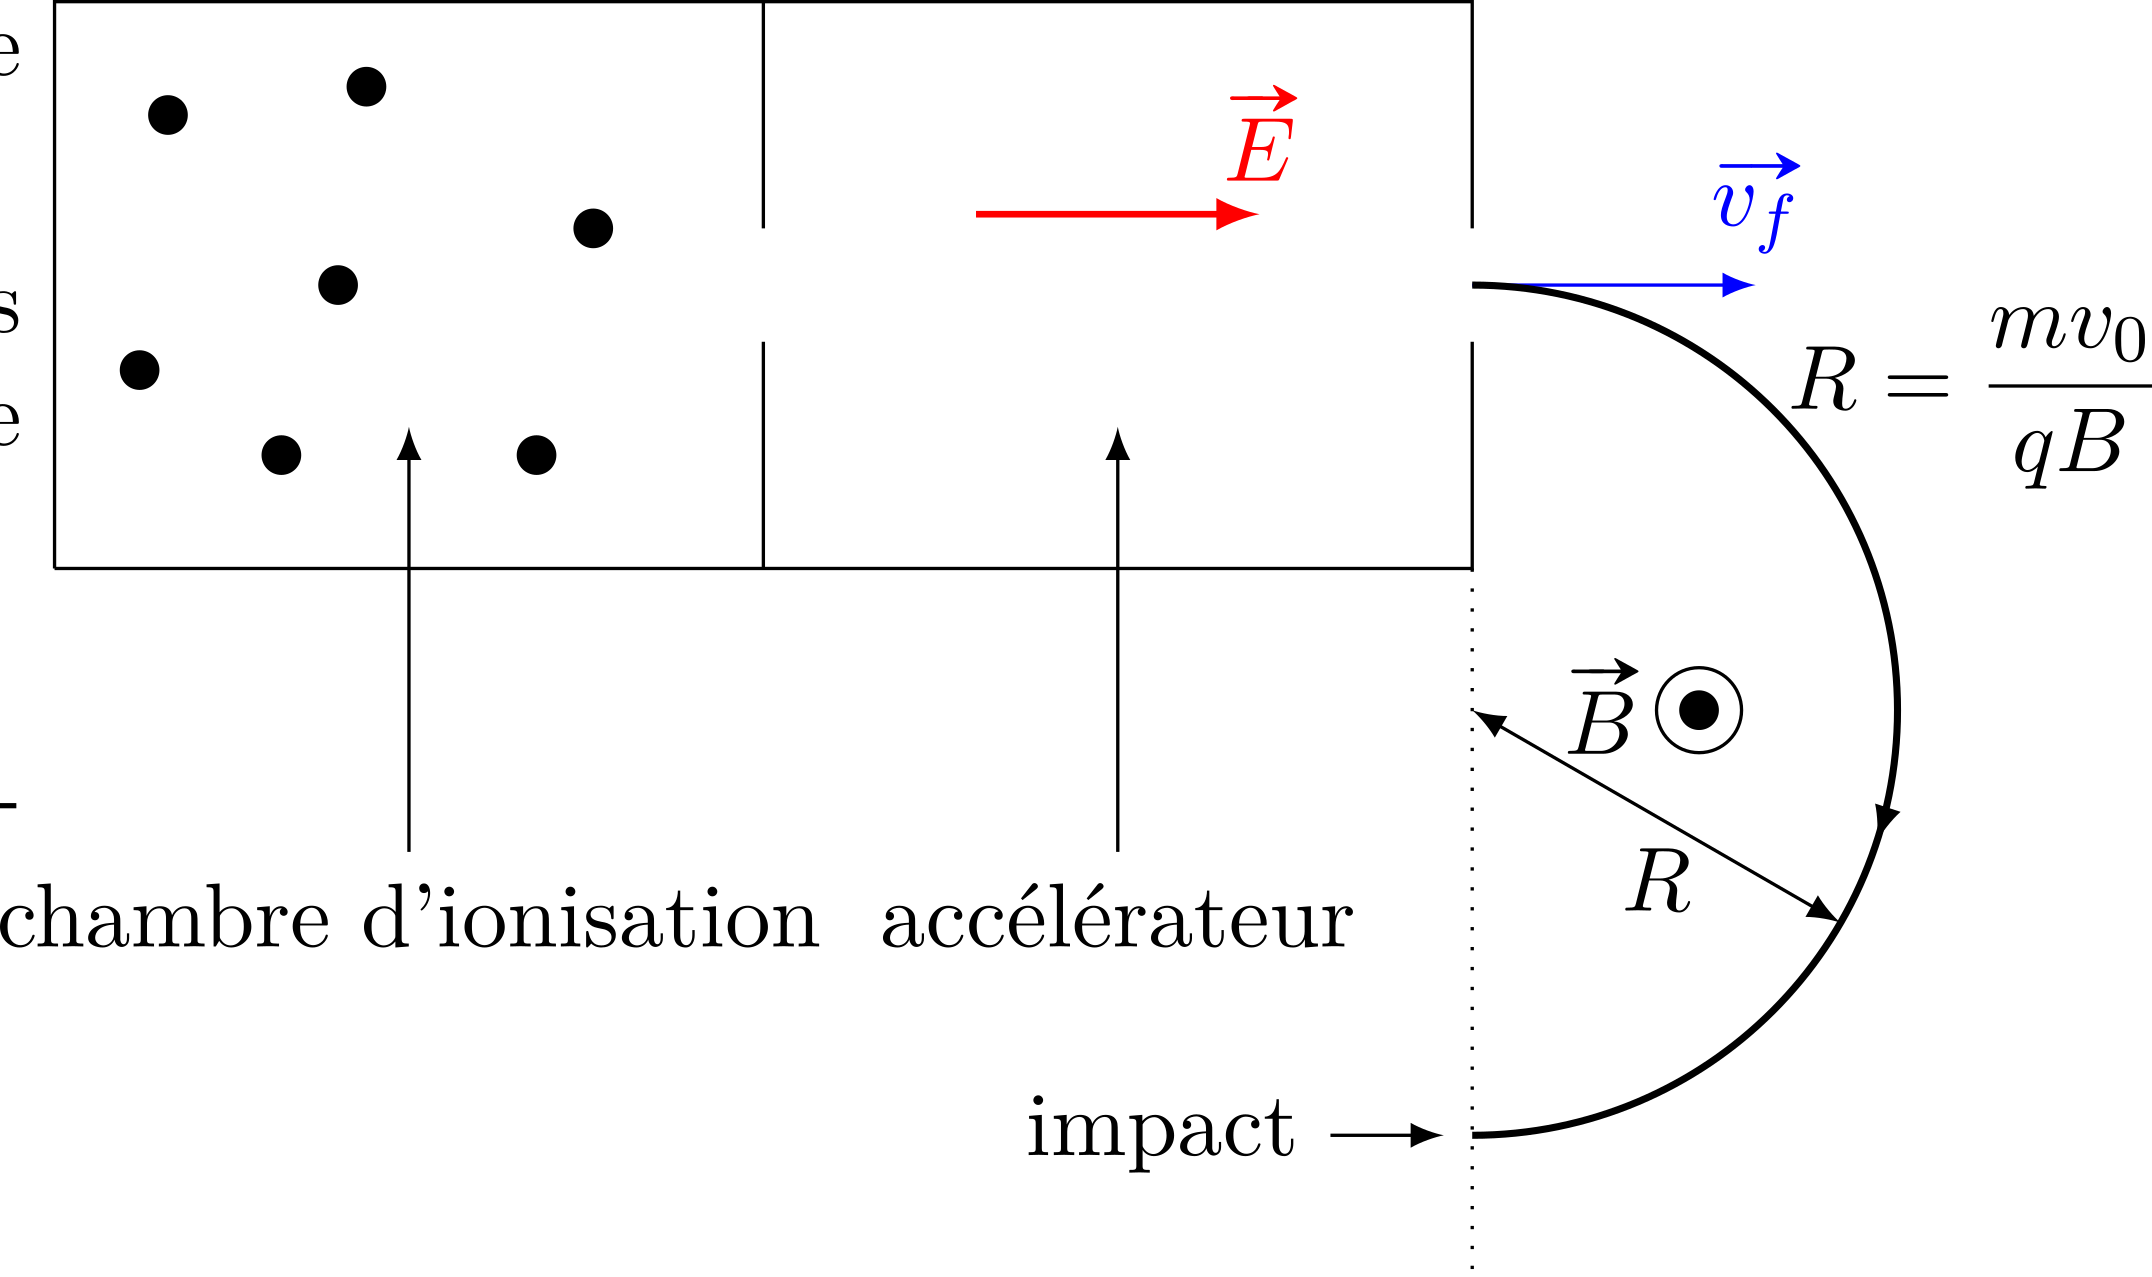
\includegraphics[width=.5\linewidth]{spectrometre}
		\captionof{figure}{Fonctionnement d'un spectromètre}
		\label{fig:spectrometre}
	\end{center}
	\begin{itemize}
		\item Des atomes sont ionisés dans une chambre d'ionisation~;
		\item Une ouverture fait sortir un flux de particules qui son
		      accélérées par un champ électrique, pour les amener à une
		      vitesse $v_f = \DS \sqrt{\frac{2qU}{m}}$~;
		\item Un champ magnétique courbe ensuite leur trajectoire, avec un
		      rayon
		      \[R_c = \frac{mv_f}{qB} = \sqrt{\frac{2qU}{m}}\frac{m}{qB} =
			      \frac{1}{B} \sqrt{\frac{2U}{q}}\sqrt{m}\]
	\end{itemize}
	Ainsi, la donnée de la distance d'impact permet de retrouver la masse
	des particules~!
	\bitem{Le cyclotron.} Il est constitué de deux demi-cylindres dans lequel
	règne un champ magnétique. Entre les deux demi-cylindres, deux
	électrodes imposent un champ électrique.
	\begin{itemize}
		\item La particule chargée est accélérée dans l'espace entre les
		      cylindres~;
		\item Elle fait demi-tour grâce à un champ magnétique qui la fait
		      revenir dans la zone entre-deux~;
		\item Avec un courant alternatif bien réglé, la tension accélère de
		      nouveau la particule~;
		\item Le champ magnétique la fait revenir, et ainsi de suite.
	\end{itemize}
	À chaque demi-tour, l'énergie cinétique croît de $\abs{qU}$. La vitesse croît
	donc comme la racine carré du nombre de passages dans l'espace entre les
	cylindres.
	\begin{center}
		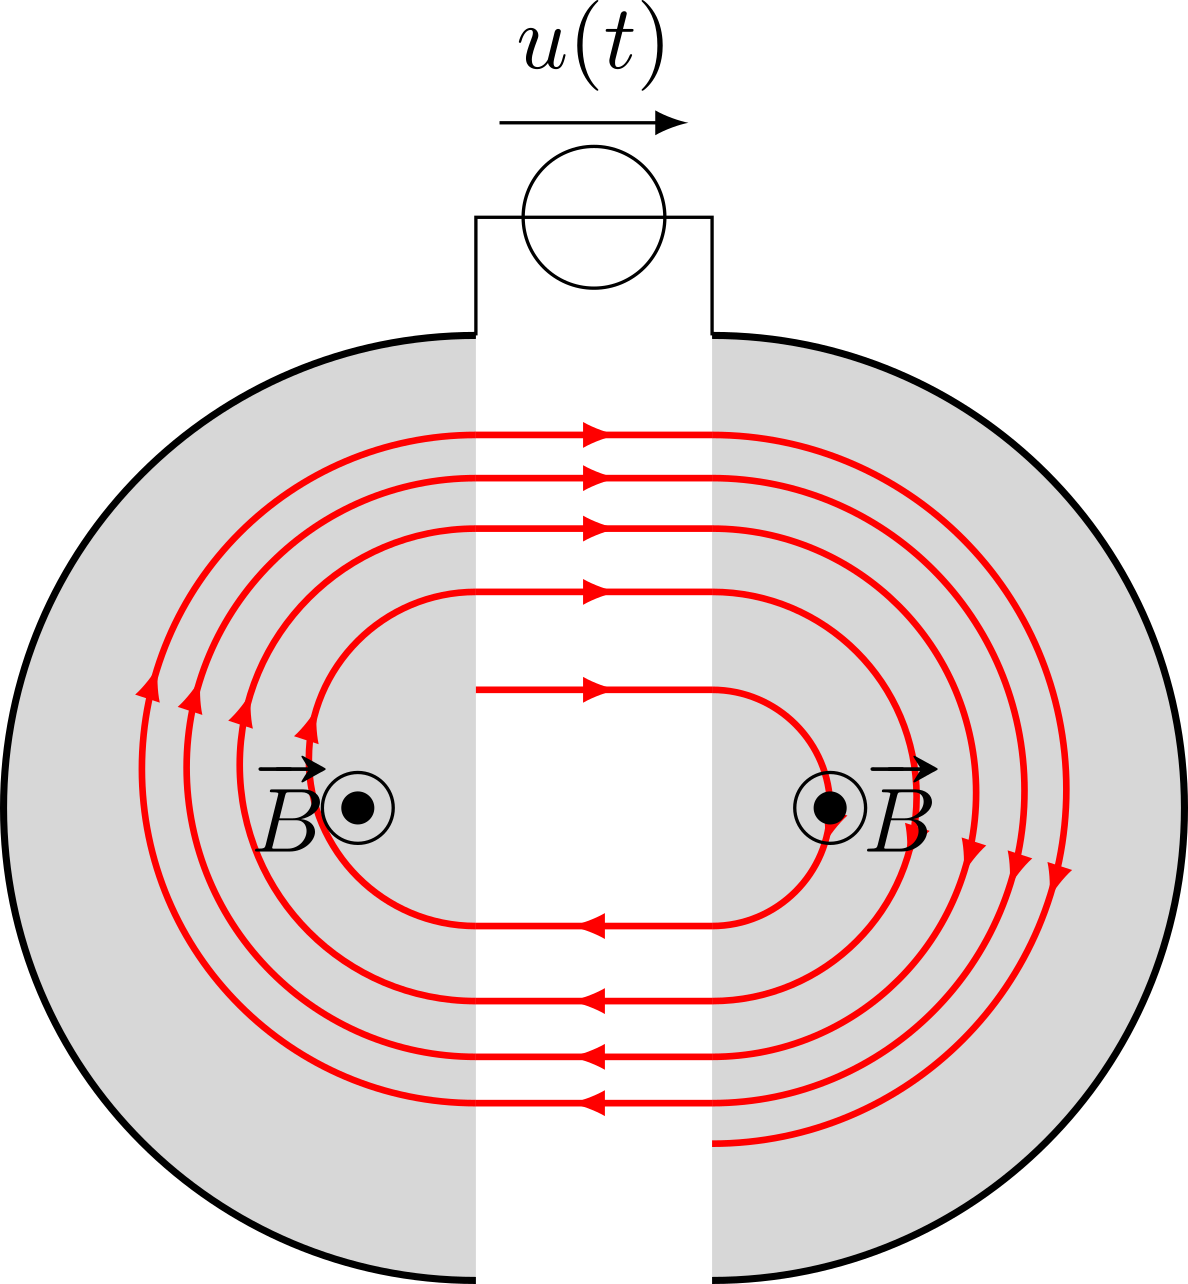
\includegraphics[scale=1]{cyclotron}
		\captionof{figure}{Fonctionnement d'un cyclotron}
		\label{fig:cyclotron}
	\end{center}
	Le rayon de courbure est proportionnel à la vitesse de la particule~: la
	sélection de ce rayon permet la sélection de l'énergie cinétique
	voulue. Voir l'animation en
	ligne\footnote{\url{http://www.sciences.univ-nantes.fr/sites/genevieve_tulloue/Meca/Charges/cyclotron.php}}.
	\bigbreak
	\bitem{L'effet \textsc{Hall}.} On considère un fil parcouru par une intensité
	$i$ vers la droite. Les électrons se déplacent en sens inverse, soit
	$\vf = -v\ux$. Si un champ magnétique est imposé selon $\uz$, ils sont
	déviés selon $-\uy$ ($q < 0$), et s'accumulent sur une paroi du fil. Un
	déséquilibre de charge s'installe, créant alors un champ appelé champ de
	\textsc{Hall}.
	\begin{center}
		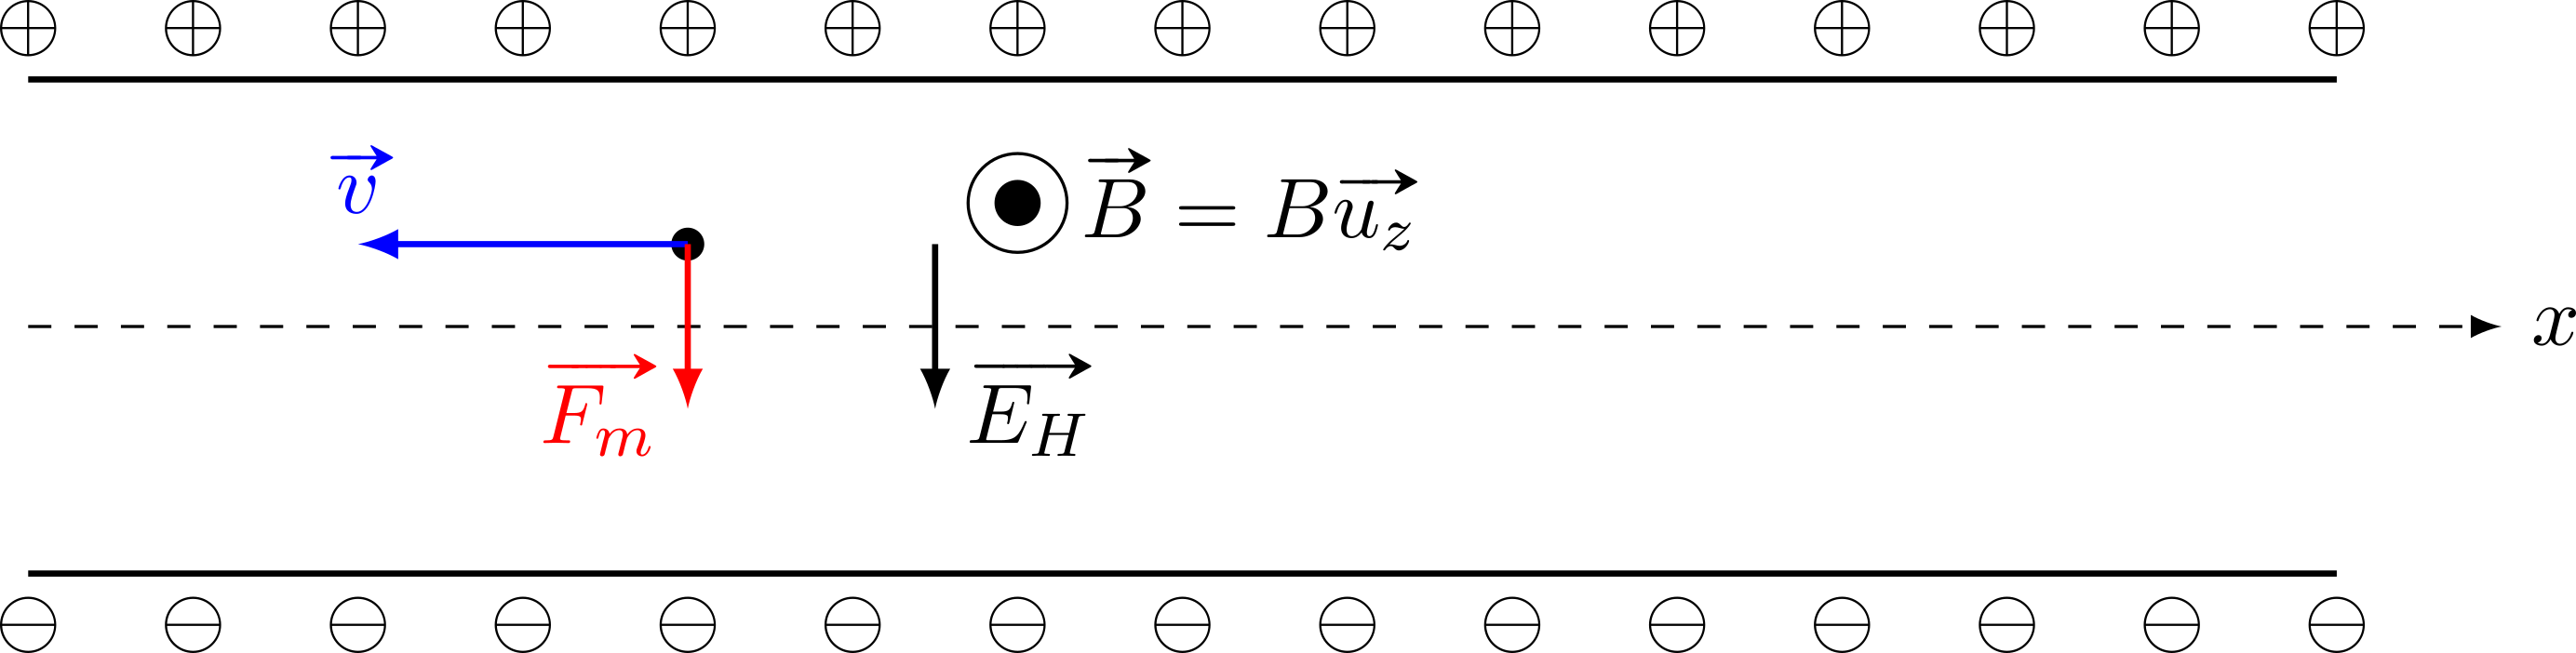
\includegraphics[scale=1]{effet_hall}
		\captionof{figure}{Effet \textsc{Hall} dans un fil}
		\label{fig:hall}
	\end{center}
	En régime permanent, la force résultant de ce champ de \textsc{Hall}
	compense la force magnétique~:
	\[
		-e\Ef_H -evB\uy = \of
		\qdonc
		\Ef_H = -vB\uz
	\]
	On mesure la tension entre la partie supérieure du conducteur et sa
	partie inférieure~:
	\[U = V(y=D) - V(y=0) = vBd\]
	Ainsi, la mesure de $U$ permet la mesure du champ $B$~! C'est le
	principe des teslamètres à effet \textsc{Hall}.
\end{itemize}

\end{document}
